% \documentclass[12pt]{scrreprt}
\documentclass[12pt]{report} 

% language may be romanian or english (default is english)
% type may be bachelor or master (default is bachelor)
\usepackage[language=english, type=bachelor]{style}

%\geometry{a4paper,top=2.5cm,left=3cm,right=2.5cm,bottom=2.5cm}
%in style
%controlling the appearance of your headers and footers
\usepackage{fancyhdr}
\usepackage{amssymb}
\usepackage{amsmath}
\usepackage{float}
\usepackage{graphicx}
\usepackage{booktabs}
\usepackage{longtable}
\usepackage{array}
\usepackage{multirow}
\usepackage{tabularx}
\usepackage{caption}
\usepackage{hyperref}
\usepackage{listings}
\usepackage{microtype}
\setlength{\emergencystretch}{3em}
\pagestyle{fancy}
\lhead{}
\chead{}
\renewcommand{\headrulewidth}{0.2pt}
\renewcommand{\footrulewidth}{0.2pt}

\begin{document}

\specialization{COMPUTER SCIENCE}	
\title{Assessment of Physical Rehabilitation
Exercises using Deep Learning and
Computer Vision}					   
\author{Alexe Nicolae-Răzvan}											
\supervisor{Conf. Dr. Bocicor Maria - Iuliana}				
				
\maketitle


\newpage


\begin{titlepage} 

\begin{center}
{\Large\textbf{
UNIVERSITATEA BABEȘ-BOLYAI CLUJ-NAPOCA \\
FACULTATEA DE MATEMATICĂ ȘI INFORMATICĂ \\
SPECIALIZAREA INFORMATICĂ \\
}}
\end{center}

\vspace{10em}

\begin{center}
{\Huge\textbf{
LUCRARE DE LICENȚĂ
}}
\end{center}

\vspace{3em}

\begin{center}
{\huge\textbf{Evaluarea exercițiilor de reabilitare
fizică folosind
Deep Learning și Computer Vision}}
\end{center}

\vspace{10em}

\begin{flushleft}
{\Large\textbf{
Conducător științific \\ Conf. Dr. Bocicor Maria - Iuliana
}}
\end{flushleft}

\vspace{3em}

\begin{flushright}
{\Large\textit{
Absolvent\\ Alexe Nicolae-Răzvan
}}
\end{flushright}

\vfill

\begin{center}
{\Large{2026}}
\end{center}

\end{titlepage}

\thispagestyle{empty}
\mbox{}
\newpage
\pagenumbering{roman} 

\cleardoublepage
ABSTRACT
\vspace{0.5cm}	
\hrule
\vspace{0.5cm}	
%\cleardoublepage

Physical rehabilitation is critical for restoring functional mobility, 
yet its efficacy is severely constrained by the lack of expert supervision 
in home environments. While automated motion assessment systems present a
 scalable solution, traditional models frequently operate as opaque "black 
 boxes," struggling with interpretability and failing to account for natural
  anthropometric variability among patients. This thesis introduces KinetoCheck,
   a comprehensive AI-assisted software platform designed to evaluate movement
    quality using standard, accessible RGB cameras. Bridging the gap between 
    complex machine learning and clinical utility, the system is deployed as
     a fully functional application offering an intuitive interface for both 
     patient execution and clinical monitoring. The underlying algorithm 
     leverages an original dual-stream deep learning architecture: one stream 
     utilizes Spatio-Temporal Graph Attention Networks (ST-GAT) to analyze 
     spatial body topology, while a 1D-CNN stream captures joint-angle temporal
      dynamics. Trained on the University of Idaho Physical Rehabilitation
       Movement Data (UI-PRMD)\cite{VJPB18}, the model employs a Siamese architecture 
       optimized via Contrastive Loss to establish a robust, subject-invariant
        standard for movement execution. 
        
        Transcending conventional binary 
        classification, KinetoCheck evaluates patients on a continuous quality
         scale and explicitly exploits graph attention weights to visually
          isolate "Joints of Attention" (JoA). This novel extraction mechanism 
          provides users with transparent, biomechanically interpretable 
          feedback regarding specific postural errors, demonstrating that 
          high-performance rehabilitation AI can be achieved without 
          sacrificing clinical transparency.

This work is the result of my own activity. I have neither given nor received unauthorized assistance on this work.
\tableofcontents


\newpage
\pagenumbering{arabic}

\chapter{Introduction}
\label{chap:introduction}

\section{Motivation}
\label{sec:intro-motivation}


Physical rehabilitation is paramount for recovering functional mobility following surgery, injury, or neurological events like stroke. However, the majority of rehabilitation protocols require patients to complete routines independently at home \cite{argent2018patient}. Without direct clinical supervision, patients frequently execute movements incorrectly, leading to suboptimal muscle engagement and an increased risk of secondary injuries. Concurrently, rapid advancements in accessible sensing technologies—such as RGBbased pose estimation and affordable depth cameras—have made the deployment of automated virtual coaching systems increasingly viable. Despite these technological strides, existing systems often fail to provide actionable, clinically relevant feedback. This thesis aims to bridge this gap by developing a system that delivers anatomically meaningful guidance, pinpointing precisely where and how movement quality degrades, rather than merely offering generic pass/fail assessments.

\section{Problem Statement}
\label{sec:intro-problem}

Automated rehabilitation assessment presents a fundamentally different computational challenge compared to generic human action recognition. While action recognition asks what action is being performed, rehabilitation assessment must determine how well that specific action is executed.
Driven by the structure of benchmark datasets \cite{VJPB18}, most existing methodologies simplify this nuanced challenge into a binary classification problem \cite{ZGAA25}, which fundamentally fails to capture the gradual, incremental progress characteristic of patient recovery. 

Furthermore, machine learning models trained on relatively small-scale rehabilitation datasets are highly susceptible to ”identity leakage.” In these instances, networks inadvertently memorize subject-specific physical characteristics (such as body proportions) rather than learning the generalized kinematic patterns of the movement itself. Consequently, these models suffer from severe performance degradation when evaluated on unseen patients. Finally, the ”black box” nature of traditional deep learning prevents clinicians from understanding why a movement was flagged as incorrect, severely limiting the clinical trust and adoption of these tools.

\section{Aims and Objectives}
\label{sec:intro-aims}

The primary aim of this thesis is to design and develop an interpretable, subjectinvariant deep learning framework for the automated quality assessment of physical rehabilitation exercises. 

To achieve this overarching goal, the research pursues the following specific objectives:

\begin{itemize}
	\item \textbf{Develop robust geometric normalization strategies} to mitigate subject-specific anthropometric bias, directly addressing the challenge of identity leakage and enabling strict cross-subject generalization (e.g., Leave-One-Subject-Out evaluation).
	\item \textbf{Design a modular feature extraction pipeline} that seamlessly transitions between baseline spatial coordinates and angle-augmented kinematic representations to capture complex temporal dynamics.
	\item \textbf{Formulate a contrastive learning paradigm}, utilizing validation-calibrated thresholding, to evaluate human movement quality on a continuous, quantifiable scale (ranging from 0 to 1), enabling the tracking of gradual patient recovery.
	\item \textbf{Generate Explainable AI (XAI) visual feedback} by mapping network attention weights back to the skeletal structure, actively highlighting the ”Joints of Attention” (JoA) to localize biomechanical errors for the user.
\end{itemize}

\section{Declaration of Generative AI and AI-assisted technologies in the writing process}
\label{sec:intro-ai-disclosure}

During the preparation of this work the author used Gemini in order to generate initial drafts of some sections, accelerating the writing process, LaTeX code formatting ( table generation and mathematical expressions) and code formatting. After using this tool/service, the author reviewed and edited the content as needed and takes full responsibility for the content of the thesis.
%\addcontentsline{toc}{chapter}{Introducere}
%\addcontentsline{toc}{chapter}{Introduction}

\chapter{State of the Art and Theoretical Background}
\label{chap:theory}

This chapter is organized into two parts. The first develops the theoretical foundations required to understand KinetoCheck, and the second reviews the most relevant prior work before synthesizing the research gaps that motivate the thesis contribution.

\section{Theoretical Foundations}
\label{sec:theory-foundations}

The following subsections introduce the conceptual building blocks used throughout the thesis.

\subsection{Motion Analysis and Human Pose Estimation}
\label{subsec:motion-analysis}

Automated assessment of rehabilitation movements depends on reliable pose acquisition and clinically meaningful temporal interpretation. Two broad families dominate current systems: marker-based motion capture and markerless visual pose estimation.

Marker-based systems, such as Vicon, estimate body kinematics from reflective markers tracked by calibrated cameras, and are generally considered high-precision in controlled laboratory settings \cite{ZGAA25}. Their primary strengths are geometric accuracy and repeatability; however, hardware cost, setup complexity, and the need for supervised capture environments reduce accessibility for home rehabilitation scenarios \cite{ZGAA25}.

Markerless systems, including MediaPipe Pose Landmarker, infer keypoints directly from RGB input and thus support low-cost, scalable deployment \cite{LTN+19,BGR+20,CSWS17}. These approaches improve practicality, but are more sensitive to occlusions, illumination variability, camera angle changes, and partial-body visibility \cite{BGR+20,CSWS17}. Consequently, a practical rehabilitation system must treat pose extraction uncertainty as a first-class design constraint.

For this thesis, the training phase relies on the UI-PRMD dataset, while deployment relies on RGB-based pose extraction. This cross-domain setup requires representation-level compatibility between high-quality motion capture trajectories and noisier in-the-wild visual keypoints. Theoretical implications include the need for invariant normalization, stable temporal resampling, and robustness-oriented feature design.

The dataset composition used in this thesis is summarized in Table~\ref{tab:T1} (see Chapter 5 for full dataset details used in experiments). 3D joint visualizations for the original Vicon and the reduced 17-joint mapping are shown in Chapter 5 Figure~\ref{fig:vicon-comparison}.

\subsection{Skeleton-Based Learning for Time Series}
\label{subsec:skeleton-learning}

Human movement can be modeled as a time-indexed sequence of articulated joint states. In this formulation, each frame is represented by a set of keypoints, and a complete repetition forms a multivariate temporal signal.

Let $T$ denote the number of time steps, $N$ the number of joints, and $C$ the coordinate dimension. A skeletal sequence is represented as:
\begin{equation}
X \in \mathbb{R}^{T \times N \times C}
\end{equation}
In rehabilitation assessment, this representation is preferred over raw RGB because it suppresses texture/background noise and emphasizes biomechanical structure \cite{ZGAA25}.

Graph modeling is a natural extension of this formulation. The body is encoded as a graph $G = (V,E)$, where nodes correspond to joints and edges to anatomical relations. This captures the non-Euclidean dependencies among body parts and enables locality-aware processing across physically connected joints \cite{CXJS22,GYDD18}. Compared with flat vector encodings, graph representations preserve meaningful topology needed to identify compensatory motion patterns.

In KinetoCheck, additional temporal features such as velocity and acceleration are used to represent execution quality beyond static posture. The theoretical motivation is that incorrect movement often manifests as trajectory irregularity or unstable timing rather than endpoint error alone.

The joint mapping used for representation alignment is summarized in Table~\ref{tab:T2_joint_mapping}.

\begin{table}[htbp]
\centering
\scriptsize
\begin{tabular}{|p{2.5cm}|p{1.5cm}|p{3.5cm}|p{2.0cm}|p{3.0cm}|p{1.5cm}|}
\hline
\textbf{Vicon Marker} & \textbf{Index} & \textbf{Target Joint} & \textbf{Target Index} & \textbf{Mapping Rule} & \textbf{Included} \\ \hline
LFHD & 1 & nose & 0 & midpoint(1,2) & Y \\ \hline
RFHD & 2 & nose & 0 & midpoint(1,2) & Y \\ \hline
LBHD & 3 &  &  & not\_used & N \\ \hline
RBHD & 4 &  &  & not\_used & N \\ \hline
C7 & 5 &  &  & not\_used & N \\ \hline
T10 & 6 &  &  & not\_used & N \\ \hline
CLAV & 7 &  &  & not\_used & N \\ \hline
STRN & 8 &  &  & not\_used & N \\ \hline
RBAK & 9 &  &  & not\_used & N \\ \hline
LSHO & 10 & left\_shoulder & 1 & direct & Y \\ \hline
LUPA & 11 &  &  & not\_used & N \\ \hline
LELB & 12 & left\_elbow & 3 & direct & Y \\ \hline
LFRM & 13 &  &  & not\_used & N \\ \hline
LWRA & 14 & left\_wrist & 5 & midpoint(14,15) & Y \\ \hline
LWRB & 15 & left\_wrist & 5 & midpoint(14,15) & Y \\ \hline
LFIN & 16 &  &  & not\_used & N \\ \hline
RSHO & 17 & right\_shoulder & 2 & direct & Y \\ \hline
RUPA & 18 &  &  & not\_used & N \\ \hline
RELB & 19 & right\_elbow & 4 & direct & Y \\ \hline
RFRM & 20 &  &  & not\_used & N \\ \hline
RWRA & 21 & right\_wrist & 6 & midpoint(21,22) & Y \\ \hline
RWRB & 22 & right\_wrist & 6 & midpoint(21,22) & Y \\ \hline
RFIN & 23 &  &  & not\_used & N \\ \hline
LASI & 24 & left\_hip & 7 & midpoint(24,26) & Y \\ \hline
RASI & 25 & right\_hip & 8 & midpoint(25,27) & Y \\ \hline
LPSI & 26 & left\_hip & 7 & midpoint(24,26) & Y \\ \hline
RPSI & 27 & right\_hip & 8 & midpoint(25,27) & Y \\ \hline
LTHI & 28 &  &  & not\_used & N \\ \hline
LKNE & 29 & left\_knee & 9 & direct & Y \\ \hline
LTIB & 30 &  &  & not\_used & N \\ \hline
LANK & 31 & left\_ankle & 11 & direct & Y \\ \hline
LHEE & 32 & left\_heel & 13 & direct & Y \\ \hline
LTOE & 33 & left\_foot\_index & 15 & direct & Y \\ \hline
RTHI & 34 &  &  & not\_used & N \\ \hline
RKNE & 35 & right\_knee & 10 & direct & Y \\ \hline
RTIB & 36 &  &  & not\_used & N \\ \hline
RANK & 37 & right\_ankle & 12 & direct & Y \\ \hline
RHEE & 38 & right\_heel & 14 & direct & Y \\ \hline
RTOE & 39 & right\_foot\_index & 16 & direct & Y \\ \hline
\end{tabular}
\caption{Joint mapping from Vicon markers to 17-joint model}
\label{tab:T2_joint_mapping}
\end{table}

\subsection{GNNs and ST-GAT for Rehabilitation Assessment}
\label{subsec:gnn-stgat}

Graph Neural Networks (GNNs) extend deep learning to structured relational data. For movement analysis, spatial-temporal graph models process inter-joint relations and time evolution, which makes them suitable for quality-sensitive exercise assessment \cite{CXJS22,GYDD18}.

Spatio-Temporal Graph Attention Networks (ST-GAT) improve over fixed-neighborhood graph convolutions by learning attention weights that adapt to exercise phase and local error context. Intuitively, not all joints are equally informative at every moment. During one phase of an exercise, knee and hip joints may dominate quality evidence, while during another phase trunk compensation may become decisive.

Formally, attention coefficients are computed from learned node projections and normalized over local neighborhoods. This mechanism gives the model adaptive selectivity while retaining graph structure. Graph attention with multi-scale temporal modeling further increases representational diversity by allowing parallel focus patterns \cite{CXJS22}.

Temporal modeling can be integrated with recurrent models (RNN/LSTM), temporal convolutional networks (TCN), or transformer-style self-attention. RNNs capture sequential context but may struggle with long dependencies and parallelization. TCNs are efficient and stable for fixed-window processing. Transformers model long-range relations but often require larger datasets and careful regularization \cite{CXJS22,GYDD18}. A temporal pyramid strategy offers a practical compromise: multiple temporal resolutions improve robustness to speed variation while maintaining manageable computational complexity.



\subsection{Siamese Networks and Pairwise Metric Learning}
\label{subsec:siamese-metric}

Usual classification predicts discrete labels. In rehabilitation, however, movement quality is often continuous and progression-oriented. Pairwise metric learning addresses this by embedding repetitions into a latent space where geometric distance reflects execution similarity \cite{BGL+93, HCL06, KZS15}.

Given two sequences $x_i$ and $x_j$, a Siamese encoder $f(\cdot)$ produces embeddings $z_i = f(x_i)$ and $z_j = f(x_j)$. A similarity score is then derived from a distance or similarity function such as cosine similarity. Contrastive objectives enforce smaller distances for similar-quality pairs and larger distances for dissimilar-quality pairs.

For the contrastive formulation used in this thesis, the model learns from pairs rather than triplets. Let $z_a$ and $z_b$ be the embeddings of a template and a user execution, and let $y \in \{0, 1\}$ indicate whether the pair is similar. A standard objective is:
\begin{equation}
\mathcal{L}_{contrastive} = y \cdot d(z_a, z_b)^2 + (1 - y) \cdot \max(0, m - d(z_a, z_b))^2
\end{equation}
where $m$ is a positive margin. Decision thresholds can then convert similarity scores into correct/incorrect predictions, while preserving the option to report confidence-like or quality-like scalar outputs.

From a theoretical perspective, this paradigm is aligned with rehabilitation goals: it supports both binary decisions for screening and graded progress tracking across sessions.

\subsection{Explainability in Movement Assessment}
\label{subsec:explainability}

Clinical usability requires not only a decision but also an explanation. Attention-based models provide one interpretable signal: joint-level importance derived from learned attention patterns. In KinetoCheck, this notion is operationalized as problematic or salient joints that contribute strongly to a low-quality decision.

Explainability in this context should be treated cautiously. High attention does not automatically imply causal biomechanical error, and visual explanations may be affected by input noise, landmark jitter, and graph connectivity assumptions \cite{JW19,AGM+18,Rud19}. Therefore, attention-based feedback is best interpreted as decision support, not as a substitute for expert diagnosis.

Actionable feedback design must satisfy three conditions: localizability (which joints), temporal context (when in the motion cycle), and readability (how users understand corrective hints). These principles motivate coupling model outputs with visual overlays and structured textual summaries in the practical system.



\section{Review of Related Work}
\label{sec:related-work}

This section surveys the most relevant movement-assessment literature and positions the thesis against it.

\subsection{Traditional Movement Assessment}
\label{subsec:rw-traditional}

Early systems for rehabilitation assessment relied on non-learning-based techniques, including Dynamic Time Warping (DTW) and Gaussian Mixture Models (GMM). While these methods were interpretable, they struggled with subject variability and lacked the capacity to learn deep hierarchical movement representations. Comparative benchmark analyses on rehabilitation datasets further motivate the transition to more expressive learned representations \cite{ZGAA25}.

\subsection{The Pioneer Deep Learning Framework (Liao et al.)}
\label{subsec:rw-liao}

The first significant deep-learning implementation for rehabilitation assessment was proposed by Liao et al. (2020) \cite{LVX20}, who introduced the UI-PRMD dataset and established a benchmark. The model introduced a Temporal Pyramid + LSTM design, where parallel 1D-CNN branches processed joint displacement signals at different time scales before temporal integration with a multi-layer LSTM. This foundational work demonstrated that hierarchical spatio-temporal modeling is essential for movement quality regression. It also highlighted the importance of multi-scale temporal representation, a principle adopted in the ST-GAT architecture used in this thesis.

\subsection{Contemporary GCN and Transformer Models}
\label{subsec:rw-contemporary}

Recent research has moved toward graph-based architectures that preserve human body topology more effectively \cite{CXJS22,GYDD18}. Notable contemporary approaches include ExeChecker (2024–2025), which introduced Joints of Attention (JoA) by extracting attention weights from STGAT backbones to provide localized feedback on problematic joints, directly influencing KinetoCheck’s interpretability design. DSTGCNT combines dense graph convolutions with GRU and Transformer components for high-accuracy quality scoring with efficient inference, exemplifying transformer-augmented spatial-temporal graph modeling \cite{CXJS22}. EGCN++ represents strong state-of-the-art performance on UI-PRMD by fusing position and orientation features \cite{yu2024egcn}. More broadly, recent analyses show that feature design and model choice remain strongly dataset-dependent \cite{ZGAA25}.

\subsection{Video-Based and Smartphone Telerehabilitation}
\label{subsec:rw-video}

Recent implementations by Chander et al. (2025) \cite{CBS25} transitioned these methods to RGB-only settings using MediaPipe \cite{LTN+19} keypoint extraction. Their results highlight the feasibility of home deployment through live repetition counting via autocorrelation and lightweight Transformer-based recognition. This work directly motivates the deployment choices made in KinetoCheck.

\section{Critical Synthesis and Research Gaps}
\label{sec:research-gaps}

Despite substantial progress in the field, three critical gaps remain unresolved. First, cross-domain consistency between laboratory motion capture and RGB-based inference remains underexplored; this thesis addresses it through systematic representation alignment. Second, many high-performing methods emphasize accuracy while providing limited clinically actionable interpretability; KinetoCheck prioritizes joint-level feedback mechanisms. Third, thresholding and score calibration strategies are often underreported, which reduces reproducibility and practical comparability across studies \cite{ZGAA25,CXJS22}.

By combining representation alignment, Siamese ST-GAT similarity learning, and interpretable joint-level feedback under strict subject-invariant evaluation protocols, this thesis contributes a comprehensive framework that addresses these gaps. The next chapter formalizes the practical system requirements and architectural design needed to realize this framework as an operational application.
% ==========================================
% CHAPTER 3: APPLICATION REQUIREMENTS
% ==========================================
\chapter{Application Requirements and System Architecture}
\label{chap:architecture}

This chapter connects the theoretical foundations from Chapter 2 with the actual implementation of KinetoCheck. It begins by turning the broad research goals and identified gaps into a concrete set of system requirements. From there, the modular architecture is introduced, breaking down the layered components and software design patterns that bring the platform to life. Together, this requirements-and-architecture blueprint sets the stage for the practical coding details and experimental results that follow.

\section{System Scope and Problem Definition}
KinetoCheck addresses the practical problem of evaluating rehabilitation exercise quality from user-provided videos, with automated feedback that is both machine-generated and interpretable. The application is designed for a semi-supervised usage scenario in which a user uploads a recording, the pipeline performs pose extraction and model inference, and the system returns a decision, score, and explanatory artifacts.

\section{System Requirements}
The system requirements are divided into functional and non-functional concerns so that the application goals and quality constraints remain explicit.

\subsection{Functional Requirements}
Functional requirements define what the application must do.
\begin{enumerate}
    \item \textbf{Video Upload:} The system shall accept a user-uploaded exercise video in supported formats: mp4, mov, mkv, avi, and webm.
    \item \textbf{Input Validation:} The system shall validate file type, file size, and basic integrity before processing.
    \item \textbf{Pose Extraction:} The system shall run MediaPipe Pose Landmarker to extract keypoints frame-by-frame from the uploaded video.
    \item \textbf{Preprocessing Consistency:} The extracted keypoints shall be transformed using the same preprocessing logic used during model training.
    \item \textbf{Inference Execution:} The system shall load the exercise-specific checkpoint and compute a similarity-based prediction.
    \item \textbf{Decision and Score Reporting:} The system shall return a predicted label (correct/incorrect), a score, and the threshold used for the decision.
    \item \textbf{Joint-Level Feedback:} The system shall identify and expose high-importance/problematic joints used for feedback visualization.
    \item \textbf{Annotated Output:} The system shall produce an annotated video or frame overlays that highlight key feedback regions.
    \item \textbf{Structured Report Export:} The system shall generate and store a JSON report containing core inference artifacts.
    \item \textbf{Analytics Summary:} The system shall generate user-level exercise statistics and overview metrics from inference outputs.
    \item \textbf{Asset Retrieval:} The web layer shall provide access to generated reports and media artifacts.
\end{enumerate}

\subsection{Non-Functional Requirements}
Non-functional requirements define quality attributes and operational constraints.
\begin{enumerate}
    \item \textbf{Reproducibility:} Given the same input and model version, the system should produce stable outputs within acceptable numerical tolerance.
    \item \textbf{Maintainability:} Training, inference, and web modules should remain separated to support independent updates.
    \item \textbf{Latency Expectation:} End-to-end processing time should be bounded for practical usability, with an acceptance target of processing time $\leq 1.0\times$ input video duration on target deployment hardware.
    \item \textbf{Robustness to Missing Detections:} The pipeline should handle partial landmark dropout through interpolation, masking, or safe fallback behavior.
    \item \textbf{Browser Compatibility:} The web layer targets the latest two stable versions of Chrome, Edge, Firefox, and Safari.
    \item \textbf{Traceability:} Each result should be linked to model version, threshold configuration, and processing timestamp.
    \item \textbf{Error Transparency:} Invalid inputs or failed processing stages should produce explicit and user-readable error messages.
    \item \textbf{Analytics Consistency:} Aggregated statistics should remain traceable to the underlying inference session, model version, and timestamp.
\end{enumerate}

The consolidated functional and non-functional requirements matrix is presented in Table~\ref{tab:T5}.


\begin{table}[H]
\centering
\small
\setlength{\tabcolsep}{4pt}
\renewcommand{\arraystretch}{1.12}
\begin{tabularx}{\textwidth}{|>{\centering\arraybackslash}p{1.2cm}|>{\centering\arraybackslash}p{0.9cm}|>{\raggedright\arraybackslash}X|>{\centering\arraybackslash}p{1.4cm}|>{\raggedright\arraybackslash}p{2.5cm}|>{\raggedright\arraybackslash}X|}
\hline
Req ID & Type & Requirement & Priority & Verification Method & Acceptance Criterion \\
\hline
F-01 & F & User shall upload a supported video file for analysis. & Must & Functional test & Valid file is accepted and processing starts. \\
F-02 & F & System shall extract 17-joint pose sequence from uploaded video. & Must & Pipeline log + output check & Sequence tensor generated with expected shape. \\
F-03 & F & System shall run checkpoint-based inference and output label/score. & Must & Functional test & Report contains predicted label, score, threshold. \\
F-04 & F & System shall generate an annotated output video. & Must & Artifact inspection & Annotated MP4 exists and is downloadable. \\
F-05 & F & System shall provide problematic-joint feedback in report. & Should & JSON schema check & worst\_joints field includes ranked entries. \\
NF-01 & NF & Pipeline shall be reproducible from scripts/configuration. & Must & Re-run reproducibility test & Comparable metrics reproduced from same checkpoint/data. \\
NF-02 & NF & System shall be maintainable with modular preprocessing/model/inference code. & Should & Code review & Clear module boundaries and documented interfaces. \\
NF-03 & NF & Inference shall tolerate temporary landmark dropouts. & Must & Robustness test & No crash; missing frames handled with fallback strategy. \\
NF-04 & NF & Web output shall be browser-compatible for video playback. & Should & Cross-browser test & Playable or downloadable output in major browsers. \\
\hline
\end{tabularx}
\caption{Functional and non-functional requirements matrix}
\label{tab:T5}
\end{table}

The requirements above define the boundaries for the implementation. The following architectural overview shows how the application components map onto those requirements.

\section{Architectural Overview}
KinetoCheck is organized as a modular pipeline that separates input acquisition, preprocessing, model inference, feedback generation, and reporting. This separation keeps the learning components independent from the application layer so that model variants can be evaluated without changing the user workflow.

\begin{figure}[H]
    \centering
    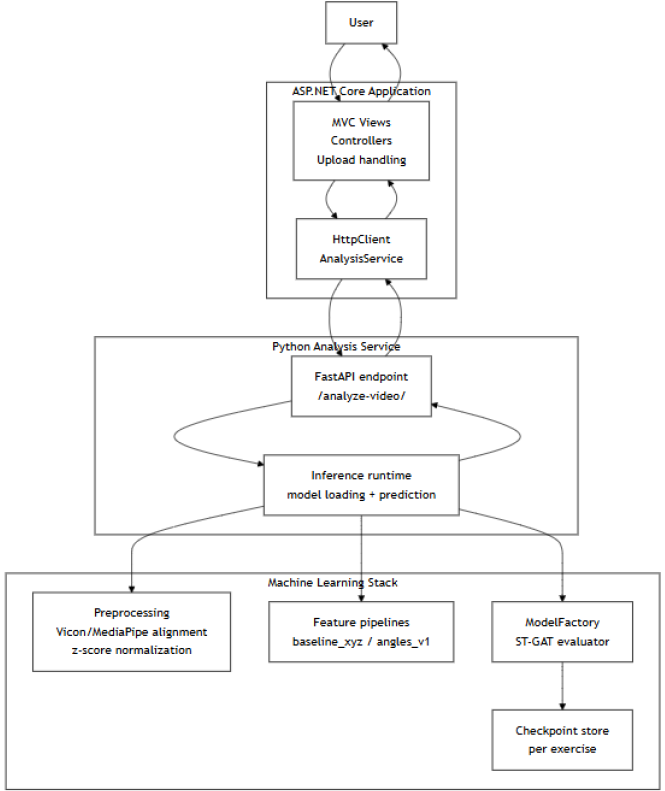
\includegraphics[width=0.9\textwidth]{figures/context_diagram.png}
    \caption{System Context Diagram depicting the separation of concerns between the presentation (ASP.NET), API (FastAPI), and machine learning layers.}
    \label{fig:system-context}
\end{figure}

The system can be summarized in five layers:
\begin{enumerate}
    \item \textbf{Input layer:} receives exercise videos, live camera streams, or dataset sequences.
    \item \textbf{Preprocessing layer:} extracts 17-joint pose sequences, aligns dataset formats, normalizes body coordinates, and constructs feature tensors.
    \item \textbf{Inference layer:} applies the ST-GAT encoder, optional phase alignment, optional frame-level decoding, and similarity scoring.
    \item \textbf{Output layer:} produces predictions, score values, and joint-level feedback for visualization.
    \item \textbf{Analytics layer:} aggregates repeated inference sessions into user-level statistics, exercise summaries, and trend reports.
\end{enumerate}

\subsection{Model and Inference Design}
The data pipeline must preserve compatibility between training and inference domains. Input video is transformed into a temporal sequence of 17-joint keypoints. The fixed tensor specification is: raw pose sequence as float32 with shape \texttt{(N, 17, 3)}, preprocessed sequence as float32 with shape \texttt{(120, 17, 3)}, and model input as float32 with shape \texttt{(B, C, 120, 17)}.

The final response package includes: prediction label and score; threshold and model identifier; problematic-joint list; annotated output media path; and JSON report path.

\begin{figure}[H]
    \centering
    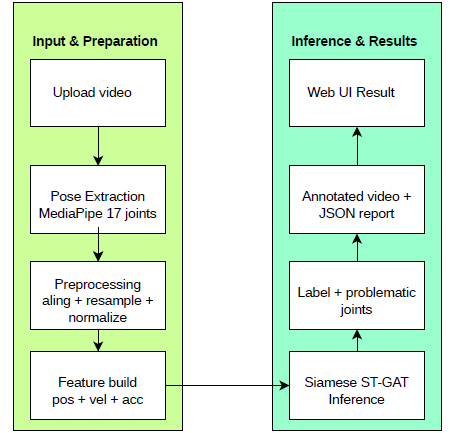
\includegraphics[width=0.6\textwidth]{figures/end-to-end.png}
    \caption{End-to-end input-output flow of the KinetoCheck application, from video upload to generated report and annotated media.}
    \label{fig:end-to-end-flow}
\end{figure}

\subsection{Data Flow and Artifact Specification}
Prediction is derived from a similarity score compared against an exercise-specific threshold. The thresholding policy must be versioned because it directly influences precision-recall behavior and user feedback interpretation. In the current implementation, threshold calibration sweeps 101 linearly spaced threshold candidates, selects the threshold that maximizes validation F1, and applies the decision rule: \texttt{correct if score >= threshold}.

To ensure reproducibility, the practical system documents the following elements:
\begin{itemize}
    \item train/validation/test partition policy (including Leave-One-Subject-Out (LOSO) if used);
    \item hyperparameter configuration and optimizer settings;
    \item checkpoint naming/versioning convention;
    \item per-exercise metrics and threshold logs;
    \item software dependencies and runtime environment.
\end{itemize}

\subsection{Analytics and Reporting Layer}
A dedicated analytics and reporting layer sits after inference and before long-term user-facing outputs. The purpose of this layer is to convert individual inference results into a longitudinal view of rehabilitation progress.

The analytics pipeline reuses existing inference artifacts instead of re-running the model. A typical session flow is:
\begin{enumerate}
    \item run exercise inference and store the score, threshold, label, and joint feedback;
    \item attach metadata such as exercise identifier, model version, and timestamp;
    \item aggregate repeated sessions by user, exercise, or time window;
    \item compute summary statistics and trend values;
    \item deliver the result to the dashboard or export it as JSON or CSV.
\end{enumerate}

\section{Software Design Patterns}

\subsection{Factory and Singleton Cache Patterns}
The factory pattern is used to create the correct evaluator implementation based on the selected checkpoint configuration. Loaded models are cached so that repeated inference requests do not reload weights from disk, reducing startup overhead.

\subsection{Composition and Component Isolation}
The phase aligner, frame decoder, and joint scorer are implemented as separate components. This keeps the architecture testable and makes it possible to improve one part of the system without rewriting the entire model stack.

This chapter has formalized both the practical requirements and the architectural design of KinetoCheck. By bridging specification and implementation design, it establishes the engineering baseline needed to interpret the training strategies and implementation details presented in the next chapter.
% ==========================================
% CHAPTER 4: TRAINING & SOFTWARE
% ==========================================
\chapter{Training Design and Software Implementation}
\label{chap:implementation}

This chapter details how the architectural requirements specified in Chapter 3 are realized through training strategies and software implementation. It first presents the training design, including the metric learning objective and the evaluation framework used to validate strict generalization. Subsequently, it describes the implementation details of key system components.

\section{Model Training Strategy}

\subsubsection*{Per-Exercise Modeling Strategy}
A foundational design choice in the KinetoCheck framework is the use of independent, exercise-specific models. Rather than training a single monolithic network to evaluate all possible movements, the pipeline trains a dedicated Siamese ST-GAT model for each of the ten exercises in the UI-PRMD dataset. This one-to-one mapping is biomechanically necessary: the optimal spatial attention weights and temporal dynamics required to evaluate a deep squat are fundamentally different from those required to evaluate a lateral lunge. By isolating the training data per exercise, each model creates a highly specialized latent space focused exclusively on the nuanced degradation patterns of that specific movement, thereby preventing cross-exercise feature interference.

The training implementation is organized around a reusable trainer and three thin entry scripts. The baseline script uses a fixed XYZ-based feature pipeline (only coordinates in the 3D cartesian space), the factory-based script allows feature extraction strategies to be selected, and the phase-aware script enables auxiliary correction outputs and Range-Of-Motion (ROM) regularization.

\begin{figure}[htbp]
    \centering
    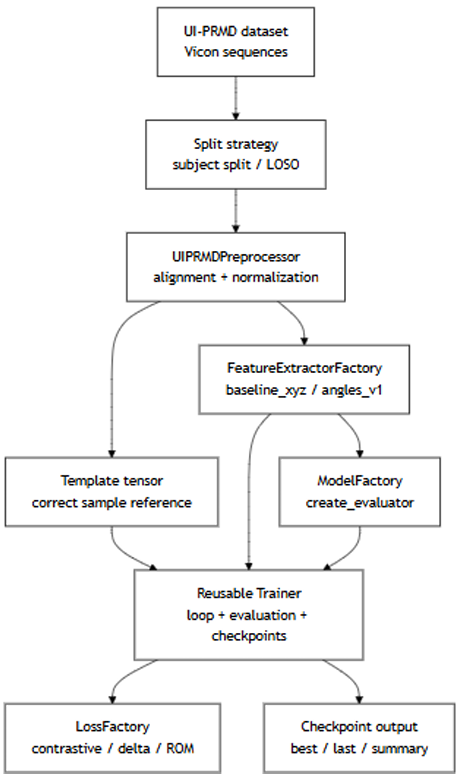
\includegraphics[width=0.9\textwidth]{figures/modular_training_architecture.png}
    \caption{The modular training architecture, highlighting the integration of the reusable trainer with feature and loss factories.}
    \label{fig:modular-training}
\end{figure}

\subsection{Spatio-Temporal Graph Attention Network Architecture}
The core processing engine of the KinetoCheck framework is the Spatio-Temporal Graph Attention Network (ST-GAT). Unlike traditional Convolutional Neural Networks (CNNs) that process dense pixel grids, or standard Recurrent Neural Networks (RNNs) that process flattened coordinate arrays, the ST-GAT preserves the explicit geometric and anatomical structure of the human body.

Building upon the theoretical graph representation established in Section 2.1.2, KinetoCheck implements the spatio-temporal graph $G$ utilizing the 17-joint MediaPipe topology. Rather than passing raw coordinates, each node $V$ is populated with the comprehensive 12-channel kinematic feature vector detailed in Section 4.2.2. The edges $E$ are strictly defined by the natural anatomical connections of the human skeleton, forming the spatial adjacency matrix used during the forward pass.

\subsubsection*{Spatial Graph Attention}
In the spatial domain, the network must understand how the movement of one joint affects its neighbors (e.g., how a collapsed knee affects the hip). Graph Attention Layers (GAT) are utilized to compute dynamic edge weights. During the forward pass, the model calculates an attention coefficient $\alpha_{i,j}$ for every pair of connected joints $i$ and $j$. This coefficient represents the biomechanical importance of joint $j$'s features to joint $i$'s current state.

This attention mechanism is the foundation of the platform’s Explainable AI (XAI) capabilities. Rather than remaining a "black box," the pooled spatial attention weights are explicitly extracted during inference and persisted into the \texttt{JointInsight} database table (as discussed in Section 4.4.2). These weights determine the Importance and Problem Score metrics, allowing the frontend to highlight specific failing joints on the user’s dashboard.

\subsubsection*{Temporal Pyramids}
Human movement occurs across multiple temporal scales simultaneously; a localized tremor might last only a few frames, while the overall repetition spans the entire sequence. To capture this without the gradient instability often associated with LSTMs, the ST-GAT implements 1D Temporal Convolutional Pyramids.

After the spatial attention layer processes the frame-wise geometry, the temporal module applies 1D dilated convolutions along the time dimension. By using parallel convolutional branches with varying receptive fields (e.g., kernel sizes of 3, 5, and 7), the network simultaneously captures high-frequency immediate anomalies (like sudden instability) and low-frequency long-term trends (like the overall speed of the repetition).

The outputs of the spatial and temporal layers are subsequently pooled into a final 128-dimensional latent embedding vector, which acts as the condensed representation of the entire exercise execution.

\subsection{Mathematical Formulation of the Contrastive Objective}
The baseline and factory-based variants optimize a contrastive loss over template and user embeddings. Rather than predicting a discrete class label, the Siamese architecture maps input sequences into a 128-dimensional latent space where the Euclidean distance between embeddings represents the biomechanical similarity of the executions.

Let $f_{\theta}(\cdot)$ denote the ST-GAT encoder parameterized by weights $\theta$. Given a template sequence $x_t$ and a user sequence $x_u$, the network generates $L_2$-normalized embeddings $z_t = f_{\theta}(x_t)$ and $z_u = f_{\theta}(x_u)$. A ground-truth label $y \in \{0, 1\}$ is provided, where $y = 1$ indicates that the user sequence is a correct execution (a positive pair), and $y = 0$ indicates an incorrect execution (a negative pair).

The optimization objective minimizes the contrastive loss function $\mathcal{L}$, defined as:
\begin{equation}
\mathcal{L}(z_t, z_u, y) = y \cdot ||z_t - z_u||_2^2 + (1 - y) \cdot \max(0, m - ||z_t - z_u||_2)^2
\end{equation}

Where:
\begin{itemize}
    \item $||z_t - z_u||_2$ is the Euclidean distance between the template and user embeddings.
    \item $m$ is the margin hyperparameter (set to 1.0 in this implementation).
\end{itemize}

During the forward pass, if the pair represents a correct execution ($y = 1$), the second term zeros out, and the network penalizes the squared distance, forcing the embeddings closer together. Conversely, if the pair is incorrect ($y = 0$), the network ignores the first term and applies a hinge loss. This hinge loss mechanism, mathematically expressed as $\max(0, m - D)$ where $D$ is the distance between embeddings, acts as a hard threshold. The margin $m$ dictates that negative pairs are only penalized if their distance is less than 1.0. Once the embeddings are pushed sufficiently far apart (i.e., $D \geq m$), the hinge loss evaluates to exactly zero, preventing the network from aggressively separating already distinct representations and thereby stabilizing the gradient updates.
This produces a continuous similarity score that is later compared against a validation-derived threshold to produce the final binary classification.

\subsubsection*{Implementation of the Contrastive Loss}
To bridge the theoretical formulation and the software architecture, the contrastive loss is implemented as a custom PyTorch module. The exact implementation used in the training pipeline is shown in Listing 4.1.

\begin{lstlisting}[language=Python, caption=PyTorch implementation of the Contrastive Loss module., label=lst:contrastive-loss, frame=single, numbers=left]
import torch
import torch.nn as nn

class ContrastiveLoss(nn.Module):
    def __init__(self, margin: float = 1.0):
        super().__init__()
        self.margin = margin

    def forward(self, emb_a: torch.Tensor, emb_b: torch.Tensor,
                labels: torch.Tensor) -> torch.Tensor:
        # Compute pairwise Euclidean distance
        distance = torch.norm(emb_a - emb_b, p=2, dim=1)

        # Loss for correct pairs (labels == 1.0)
        loss_correct = labels * torch.pow(distance, 2)

        # Loss for incorrect pairs (labels == 0.0)
        loss_incorrect = (1.0 - labels) * torch.pow(
            torch.clamp(self.margin - distance, min=0.0), 2
        )

        # Return mean loss over the batch
        return torch.mean(loss_correct + loss_incorrect)
\end{lstlisting}

As seen in Listing~\ref{lst:contrastive-loss}, the embeddings are processed in parallel batches. The \texttt{torch.norm} function computes the L2 distance across the embedding dimension (\texttt{dim=1}). The \texttt{torch.clamp} function elegantly applies the hinge mechanism for incorrect pairs, ensuring that gradients are only propagated if the distance is smaller than the configured margin. This modular design allows the \texttt{LossFactory} to instantiate the loss function dynamically based on the chosen training configuration.

\section{Data Processing and Normalization}

\subsection{Identity Leakage Mitigation}
To reduce identity leakage, subject-wise split strategies are used so that no subject appears in more than one split. The codebase also includes explicit Leave-One-Subject-Out (LOSO) utilities for stricter generalization evaluation. In preprocessing, pose sequences are centered and normalized consistently so that training and inference use the same representation.

\subsection{Kinematic Feature Engineering and 12-Channel Representation}
Raw spatial coordinates are often insufficient to fully capture the dynamic nature of physical rehabilitation exercises. To provide the ST-GAT model with a comprehensive understanding of movement biomechanics, the preprocessed 3D coordinates are expanded into a 12-channel feature representation prior to inference. For each joint at every time step, the following kinematic features are computed:

\begin{itemize}
    \item \textbf{Channels 1--3 (Spatial Position):} The normalized X, Y, and Z coordinates of the joint.
    \item \textbf{Channels 4--6 (Velocity):} The first-order temporal derivative of the position, representing the instantaneous speed and direction of the joint.
    \item \textbf{Channels 7--9 (Acceleration):} The second-order temporal derivative of the position, indicating changes in movement speed and highlighting jitter or instability.
    \item \textbf{Channel 10 (Joint Angle):} The angle formed between anatomically connected adjacent joints (e.g., the angle at the elbow formed by the shoulder and the wrist).
    \item \textbf{Channel 11 (Angular Velocity):} The temporal derivative of the joint angle, capturing the speed of rotation during the execution of the movement.
    \item \textbf{Channel 12 (Normalized Bone Length):} The distance between connected joints, normalized by the length of the torso (computed as the distance between the left hip and the left shoulder).
\end{itemize}

By incorporating velocity and acceleration alongside static position, the model successfully captures trajectory irregularities and unstable timing, which are primary indicators of poor execution quality. Furthermore, the inclusion of normalized bone ratios ensures that the resulting feature space remains robust against natural variations in subject height, body proportions, and camera distance.

\subsection{Phase-Aware Variant and Auxiliary Multi-Task Learning}
While the baseline ST-GAT encoder effectively classifies overall movement quality, clinical rehabilitation requires granular feedback regarding partial-range executions and localized joint errors. To address this, the phase-aware variant transforms the network into a multi-task learning architecture by appending two auxiliary prediction heads to the latent embedding: a Range of Motion (ROM) regularizer and a Frame Decoder.

\subsubsection*{Range of Motion (ROM) Regularization}
Patients often compensate for muscle weakness by terminating a movement prematurely. The ROM penalty continuously measures the maximum spatial displacement (amplitude) of the user’s joints and compares it against the expected amplitude of the expert template. If a user sequence is labeled as incorrect due to a truncated range of motion, the ROM penalty applies a secondary gradient update, explicitly teaching the spatial attention layers to penalize incomplete joint trajectories.

\subsubsection*{Frame-Level Error Decoding}
To further enhance the Explainable AI (XAI) capabilities, a Multi-Layer Perceptron (MLP) Frame Decoder is attached to the user embedding. This decoder projects the 128-dimensional latent representation into a 17-dimensional vector, attempting to explicitly predict the localized spatial error magnitude at each joint. This is optimized using a Mean Squared Error (MSE) loss against the ground-truth spatial delta ($\Delta X$) between the user and the aligned template.

\subsubsection*{Composite Loss Formulation}
The total multi-task loss $\mathcal{L}_{total}$ is calculated as a weighted sum of the primary contrastive objective and the two auxiliary penalties:

\begin{equation}
\mathcal{L}_{total} = \mathcal{L}_{contrastive} + \lambda_{rom} \cdot \mathcal{L}_{ROM} + \lambda_{delta} \cdot \mathcal{L}_{delta}
\end{equation}

Where $\lambda_{rom}$ and $\lambda_{delta}$ are the configurable hyperparameter weights assigned to the auxiliary objectives (detailed in Table~\ref{tab:T3}).

Benefits of this phase-aware multi-task design include:
\begin{itemize}
    \item \textbf{Targeted Supervision:} The auxiliary gradients force the network to learn correction-aware spatial representations, improving the accuracy of the extracted attention weights.
    \item \textbf{Reduced False Positives:} ROM regularization prevents the model from accidentally validating partial-range executions that otherwise maintain correct anatomical posture.
    \item \textbf{Rich Metadata:} The decoder outputs are persisted directly into the checkpoint, enabling the advanced joint-level feedback extraction (the \texttt{JointInsight} entity) utilized during inference.
\end{itemize}

Table~\ref{tab:T3} summarizes the key hyperparameters and training choices used for the reported experiments. For reproducibility, per-fold checkpoints are saved, and the training and validation splits used for each fold are stored.

\begin{table}[H]
\centering
\small
\begin{tabular}{|p{1.5cm}|p{3.5cm}|p{2.0cm}|p{2.0cm}|p{5.0cm}|}
\hline
\textbf{Group} & \textbf{Parameter} & \textbf{Value} & \textbf{Unit/Range} & \textbf{Comment} \\ \hline
model & \texttt{in\_channels} & 9/12 & channels & xyz(+velocity+acceleration) \\ \hline
model & \texttt{hidden\_channels} & (64, 128) & tuple & ST-GAT blocks \\ \hline
model & \texttt{embedding\_dim} & 128 & dim & Siamese projection head \\ \hline
model & \texttt{use\_phase\_decoder} & True & boolean & Enables temporal alignment module \\ \hline
optimizer & \texttt{learning\_rate} & 1e-3 & & Initial learning rate \\ \hline
optimizer & \texttt{weight\_decay} & 1e-4 & & L2 regularization penalty \\ \hline
optimizer & \texttt{margin} & 1.0 & & Contrastive loss margin \\ \hline
training & \texttt{delta\_weight} & 0.0 & & Frame-level correction loss weight \\ \hline
training & \texttt{rom\_weight} & 2.0 & & Range-of-motion loss weight \\ \hline
data & \texttt{batch\_size} & 8 & samples & Training batch size \\ \hline
data & \texttt{num\_workers} & 0 & threads & DataLoader workers \\ \hline
training & \texttt{epochs} & 30 & epochs & Maximum training epochs \\ \hline
training & \texttt{patience} & 10 & epochs & Early stopping patience \\ \hline
training & \texttt{seed} & 42 & & Random seed for reproducibility \\ \hline
training & \texttt{device} & auto & & Hardware accelerator \\ \hline
split & \texttt{split\_mode} & subject & & Determines data partitioning strategy \\ \hline
split & \texttt{train/val/test ratio} & 0.8/0.1/0.1 & ratio & Dataset split proportions \\ \hline
\end{tabular}
\caption{Model hyperparameters and training settings}
\label{tab:T3}
\end{table}

\subsection{Temporal Interpolation and Spatial Anchoring}
A fundamental challenge in automated movement assessment is temporal and spatial misalignment. A patient recovering from an injury will inherently execute a repetition at a different speed and possess different anatomical proportions compared to the healthy expert template. If the system were to compute error margins on a rigid, unaligned basis, a perfectly executed but slower movement would be severely penalized.

To resolve this and generate an intuitive visual overlay (the "ghost" skeleton), KinetoCheck implements a deterministic, dual-stage alignment module consisting of Linear Temporal Interpolation and Spatial Anchoring.
Before computing the temporal alignment, the system must deterministically select the baseline expert template ($T_t$) from the UI-PRMD dataset. To ensure the template reflects a natural, therapeutic execution speed, the pipeline filters all correct executions (label = 0) for a given exercise and selects the specific sequence possessing the median frame length. This dynamically extracted 'Golden Template' serves as the anchor for both the Siamese network comparison and the visual Ghost Skeleton overlay.
\subsubsection*{Linear Temporal Sequence Interpolation}
Given a user kinematic sequence of length $T_u$ and a template sequence of length $T_t$, the system maps the discrete time indices of the user's execution into the continuous temporal space of the template. For each user frame $i \in \{0, \dots, T_u - 1\}$, the corresponding fractional template index $t_i$ is computed via linear spacing:

\begin{equation}
t_i = i \cdot \frac{T_t - 1}{T_u - 1}
\end{equation}

Because $t_i$ is a continuous floating-point value, the exact template posture must be approximated using 1D linear interpolation. By isolating the lower bound index $idx_0 = \lfloor t_i \rfloor$ and the upper bound index $idx_1 = \min(idx_0 + 1, T_t - 1)$, the fractional remainder $\alpha = t_i - idx_0$ acts as a blending weight. The temporally aligned template frame $\hat{X}_t^{(i)}$ is thus computed as a weighted combination of two adjacent expert frames:

\begin{equation}
\hat{X}_t^{(i)} = (1 - \alpha) \cdot X_t^{(idx_0)} + \alpha \cdot X_t^{(idx_1)}
\end{equation}

This continuous temporal scaling ensures the ghost skeleton remains perfectly synchronized with the user's kinematic progression throughout the entire duration of the exercise, regardless of execution speed.

\subsubsection*{Spatial Anchoring and Proportional Scaling}
Once temporally synchronized, the template must be spatially normalized to match the user's specific body metrics and camera distance. The system calculates a global scaling factor $S$, derived from the median vertical distance between the distal anatomical points (the nose and the feet) across both sequences:

\begin{equation}
S = \max \left(0.5, \min \left(4.0, \frac{\text{median}(Height_{user})}{\text{median}(Height_{template})}\right)\right)
\end{equation}

Finally, a biomechanical fulcrum (such as the midpoint between the left and right hips, or the ankles) is selected as a translation anchor $A$. The temporally interpolated template frame $\hat{X}_t^{(i)}$ is centered around its own anchor, scaled by the factor $S$, and translated to match the user's spatial anchor coordinates in the 2D plane:

\begin{equation}
Ghost^{(i)} = (\hat{X}_t^{(i)} - A_{template}^{(i)}) \cdot S + A_{user}^{(i)}
\end{equation}

This combined spatio-temporal alignment allows the rendering engine to project a highly accurate, anatomically proportional, and time-locked corrective overlay directly onto the user's video feed.

\section{Pipeline Implementation}

\subsection{Video-Based Inference via MediaPipe}
For RGB input, the system uses MediaPipe Pose Landmarker to extract frame-wise 17-joint landmarks. The model infers 33 landmarks per frame; these are remapped to the 17-joint representation used during training via a deterministic mapping defined in the preprocessing layer.

\subsection{Feedback Visualization}
To expose model reasoning, the visualization module overlays the extracted skeleton on the input video and highlights the joints that are most relevant to the model output. This produces intuitive corrective cues for users and therapists.

At startup, the inference module caches loaded checkpoints in memory to avoid repeated disk I/O. Given a preprocessed pose sequence of shape \texttt{(1, C, 120, 17)}, the inference function: (1) builds the selected feature representation; (2) passes the tensor through the evaluator; (3) computes a similarity score; (4) compares the score against the learned threshold to produce a binary decision; and (5) returns a structured result object.

\subsubsection*{Spatio-Temporal Rendering and the Ghost Skeleton Overlay}
To maximize the clinical interpretability of the system, a “ghost skeleton” overlay was implemented. This visual artifact superimposes a semi-transparent representation of the optimal template movement directly onto the user’s video feed.

The geometric scaling and frame-synchronization of this overlay are handled by the deterministic alignment module detailed previously in 4.2.4. However, applying this math to in-the-wild videos introduces a final rendering challenge: Dynamic Camera Orientation Detection. Because home rehabilitation videos exhibit varying camera angles, hardcoding the lateral axis often leads to distorted 2D projections. The rendering engine automatically resolves this by measuring the shoulder separation across the X and Y dimensions, selecting the axis with the maximum geometric variance to correctly orient the template before applying the spatial anchoring equations.

This advanced rendering pipeline ensures that patients receive real-time, proportionally accurate visual cues, clearly illustrating the spatial delta between their current posture and the idealized target movement without suffering from temporal desynchronization.

\section{Application Integration}
The ASP.NET Core web interface orchestrates the request lifecycle: upload, validation, forwarding of the video to the Python analysis service, and response rendering.

\subsection{Web Interface and Request Orchestration}
\begin{enumerate}
    \item \textbf{Upload:} User selects a video file; the interface validates MIME type and file size.
    \item \textbf{Temporary Storage:} The video is written to a temporary directory with a UUID-based filename.
    \item \textbf{Pose Extraction:} MediaPipe is invoked; keypoints are logged.
    \item \textbf{Preprocessing:} Keypoints are normalized and resampled.
    \item \textbf{Inference:} The pre-trained model is loaded and a prediction is computed.
    \item \textbf{Visualization:} An annotated video is generated.
    \item \textbf{Report Generation:} A JSON report is written containing core artifacts.
    \item \textbf{Response:} The user is provided with the predicted label, score, report path, and video link.
\end{enumerate}

\begin{figure}[H]
    \centering
    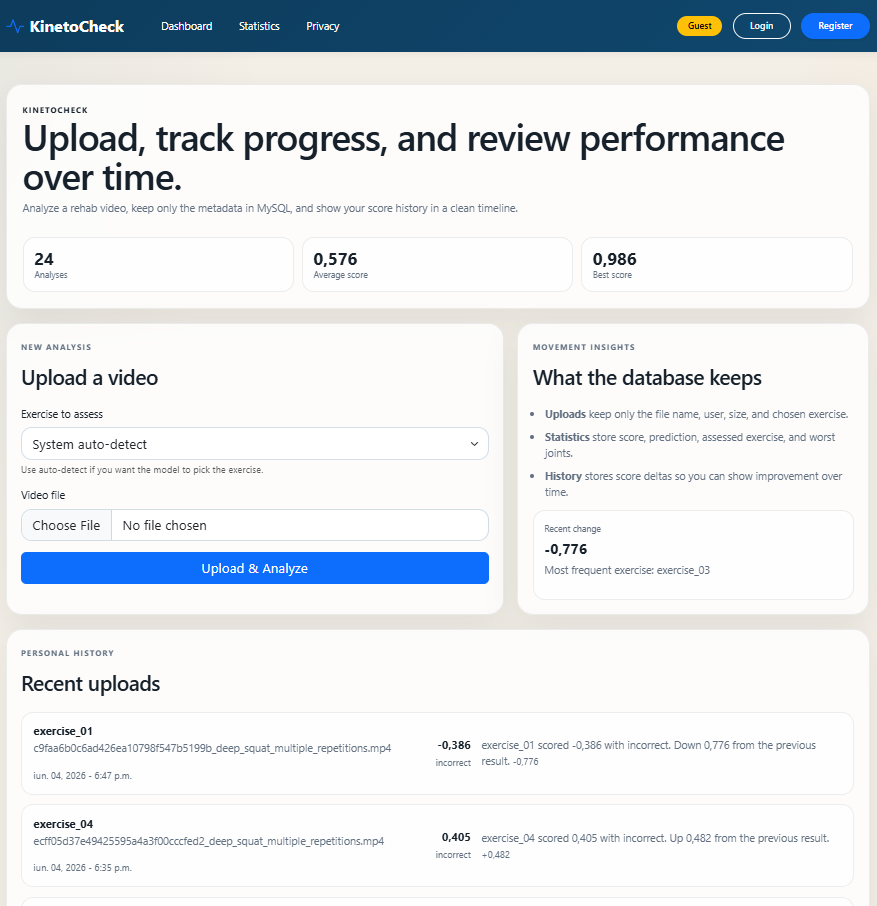
\includegraphics[width=0.9\textwidth]{figures/app_dashboard.png}
    \caption{The primary user dashboard, featuring the updated navigation bar, historical statistics, and the video upload interface.}
    \label{fig:app-dashboard}
\end{figure}

The application is designed to handle multiple concurrent requests, with asynchronous processing and caching of model checkpoints to optimize performance. Error handling is implemented at each stage to ensure that users receive informative feedback in case of issues such as invalid file formats or inference errors.

\begin{figure}[hbtp]
    \centering
    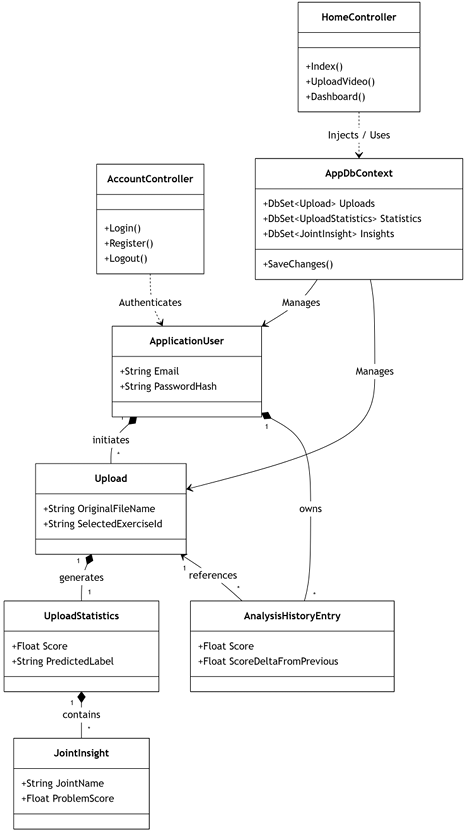
\includegraphics[width=0.8\textwidth]{figures/uml-diagram.png}
    \caption{ UML Class Diagram illustrating the core domain entities, data persistence layer, and primary web controllers.
}
    \label{fig:uml-diagram}
\end{figure}

\subsection{Data Model and Persistence (Entity Framework Core)}
Although the processing core of the KinetoCheck platform relies on deep learning models, the system operates as a comprehensive web application, requiring a robust architecture to store patient data and medical rehabilitation history. Data persistence within the .NET application is managed via Entity Framework (EF) Core. This modern Object-Relational Mapper (ORM) facilitates interaction with the relational database directly through C\# objects (via the \texttt{AppDbContext}), eliminating the need for manual SQL query construction.

To ensure strict traceability of patient progress and the decisions made by the AI model, the database was designed following normalization principles and is structured around five primary entities (illustrated in figure \ref{fig:db-diagram}):
\begin{figure}[H]
    \centering
    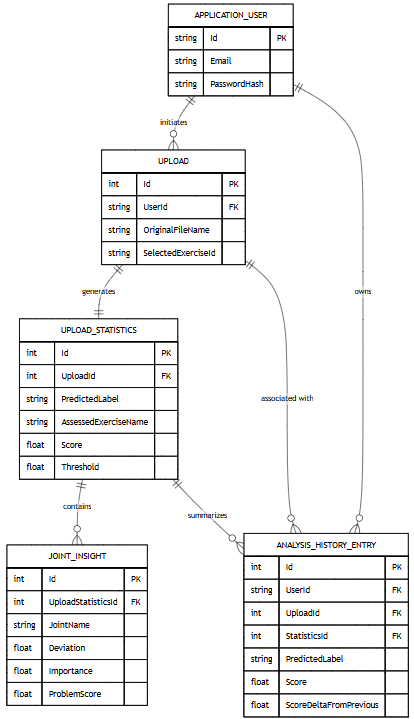
\includegraphics[width=0.7\textwidth]{figures/db-diagram.png}
    \caption{ Database Diagram illustrating the core domain entities and their relationships, as implemented via Entity Framework Core.
}
    \label{fig:db-diagram}
\end{figure}
\begin{itemize}
    \item \textbf{\texttt{ApplicationUser}:} Extends the base \texttt{IdentityUser} class from ASP.NET Core Identity. It manages profile data and account security (e.g., encrypted password hashes, session management). By utilizing the \texttt{DeleteBehavior.SetNull} constraint, the system prevents the accidental cascading deletion of aggregated medical data if a user account is ever deactivated.
    \item \textbf{\texttt{Upload}:} Represents the data entry point into the system. It stores the metadata of the original video file (\texttt{OriginalFileName}) and the identifier of the specific exercise selected by the user (\texttt{SelectedExerciseId}).
    \item \textbf{\texttt{UploadStatistics}:} Stores the raw inference results returned by the Python API in a strict one-to-one relationship with the \texttt{Upload} entity. This table captures the similarity score (\texttt{Score}), the model’s decision (\texttt{PredictedLabel}), and the automatically calibrated decision boundaries (\texttt{Threshold}, \texttt{Margin}). Isolating this data ensures rapid query execution without overloading the primary table.
    \item \textbf{\texttt{JointInsight}:} This entity is paramount for the system’s Explainable AI (XAI) capabilities. It maintains a one-to-many relationship with \texttt{UploadStatistics} and granularly stores the biomechanical errors detected at each individual joint (e.g., \texttt{Deviation}, \texttt{Importance}, \texttt{ProblemScore}). The frontend consumes this data to visually highlight problem areas (Joints of Attention) on the patient’s skeleton.
    \item \textbf{\texttt{AnalysisHistoryEntry}:} Acts as a longitudinal (time-series) evolution log. Beyond storing a textual \texttt{Summary}, it captures the \texttt{ScoreDeltaFromPrevious} metric, which automatically calculates the performance difference compared to the user’s previous execution of the same exercise. This feature is essential in a clinical context, allowing for the objective quantification of recovery progress over time.
\end{itemize}

The model utilizes strict Fluent API constraints—such as \texttt{MaxLength} and \texttt{Precision(6, 3)}—to optimize the database’s memory footprint while ensuring the strict decimal precision required by the machine learning outputs.

\subsection{Authentication and MVC Architecture}
To guarantee the confidentiality of medical data, the platform integrates a comprehensive authentication and authorization module. The entire user interaction flow is built upon the Model-View-Controller (MVC) design pattern, native to the ASP.NET Core environment.

\subsubsection*{Authentication and Access Restriction}
Access to the video analysis functionalities and medical history is strictly restricted to authenticated users. The login system, managed by the \texttt{AccountController}, employs secure Cookie Authentication to maintain active user sessions across HTTP requests. When an unauthenticated user attempts to access a protected route marked with the \texttt{[Authorize]} attribute, the security middleware automatically intercepts the request and redirects the client to the login page, thereby preventing the exposure of sensitive data.

\begin{figure}[htbp]
    \centering
    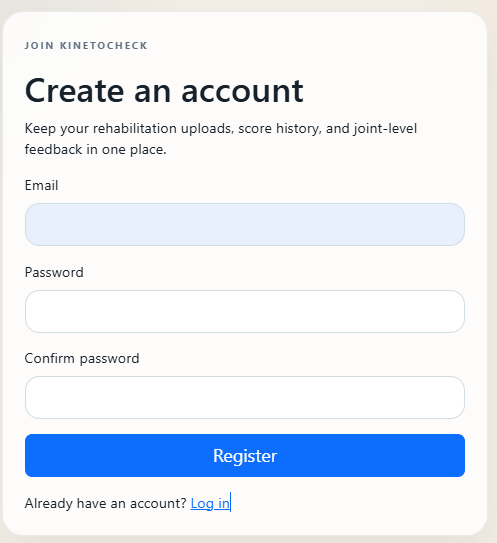
\includegraphics[width=0.7\textwidth]{figures/app_login.png}
    \caption{The KinetoCheck authentication interface, ensuring that medical analysis history remains secure and accessible only to registered users.}
    \label{fig:app-login}
\end{figure}

\subsubsection*{The Lifecycle of an Analysis Request (MVC)}
Communication between the patient and the artificial intelligence service is elegantly orchestrated through the three components of the MVC architecture:

\begin{enumerate}
    \item \textbf{View (Graphical Interface):} The frontend is constructed using Razor Pages (HTML5 with embedded C\#). The interface includes client-side validation to ensure correct file formatting before data is transmitted to the server, preserving bandwidth and preventing unnecessary backend processing.
    \item \textbf{Controller:} The application logic is cleanly separated into dedicated controllers. While the \texttt{AccountController} handles security and the \texttt{SamplesController} manages reference data, the \texttt{HomeController} acts as the primary orchestrator for the analysis pipeline. It receives the video upload from the View, temporarily stores it, and initiates an asynchronous HTTP request to the Python analysis API (FastAPI). The asynchronous nature of this call (\texttt{async/await}) is critical, allowing the .NET server thread to remain responsive and serve other users while waiting for the neural network to finish its compute-heavy operations.
    \item \textbf{Model:} Once the JSON response is returned by the AI service, the \texttt{HomeController} deserializes the payload. The data is mapped to the previously established database entities (such as \texttt{UploadStatistics} and \texttt{JointInsight}), persisted via Entity Framework Core, and the final View is rendered to display the results and the annotated ghost skeleton to the patient, thereby completing the feedback loop.
\end{enumerate}

\subsection{Error Handling and Robustness}
The implementation follows the error handling specification from Chapter 3. Key error scenarios include: invalid video input, insufficient pose quality, checkpoint mismatch, and timeout conditions. For each scenario, the system provides user-friendly error messages and avoids producing ambiguous partial outputs.

\begin{figure}[htbp]
    \centering
    
\includegraphics[width=0.8\textwidth]{figures/app_error_handling.png}
    \caption{UI error message for missing human subjects.}
    \label{fig:app-error}
\end{figure}

\begin{figure}[htbp]
    \centering
    
\includegraphics[width=0.8\textwidth]{figures/missing_human_error_handling.png}
    \caption{UI error message for image uploads.}
    \label{fig:missing-human-error}
\end{figure}
% ==========================================
% CHAPTER 5: EXPERIMENTS & RESULTS
% ==========================================
\chapter{Experiments and Results}
\label{chap:experiments}

This chapter presents the empirical validation of the KinetoCheck framework through quantitative and qualitative analyses. It documents the experimental setup, reports performance metrics comparing baseline, phase-aware, and ROM-regularized variants, and provides ablation studies to isolate the contribution of each architectural component.

\section{Experimental Setup and Protocol}
The experiments reported in this chapter follow the subject-wise split protocol described in Chapter 4, where subjects are assigned to non-overlapping train, validation, and test sets. To validate strict generalization under more demanding conditions, Leave-One-Subject-Out (LOSO) evaluation is also performed as noted below.

\subsection{Dataset Characteristics}
The UI-PRMD dataset contains 1,980 sequences across 10 subjects and 10 exercises, with a balanced distribution of correct and incorrect executions. Each subject performs each exercise multiple times, resulting in a rich set of movement variations. The dataset is captured using a Vicon motion capture system, providing high-fidelity 3D joint coordinates. The 39-joint Vicon captures are mapped to a 17-joint representation consistent with MediaPipe’s output, as illustrated in Figure~\ref{fig:vicon-comparison}.

\begin{figure}[H]
    \centering
    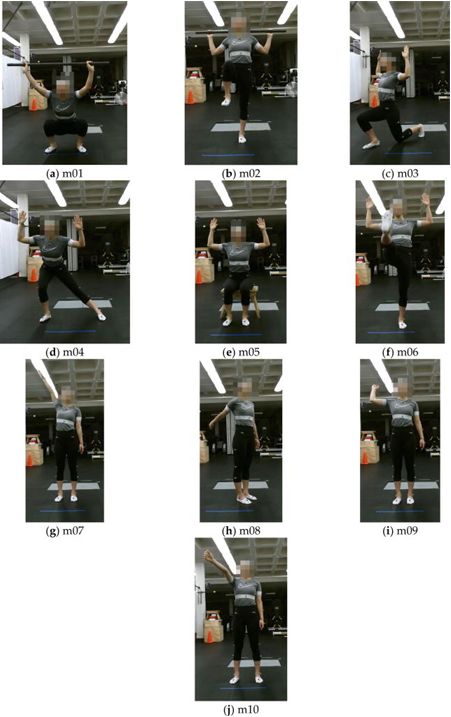
\includegraphics[width=0.75\textwidth]{figures/uiprmd_exercises.png}
    \caption{UI-PRMD exercises visualization. \cite{VJPB18}}
    \label{fig:uiprmd-visualization}
\end{figure}

\begin{table}[htbp]
\centering
\small
\setlength{\tabcolsep}{5pt}
\renewcommand{\arraystretch}{1.15}

\begin{tabularx}{\textwidth}{|>{\centering\arraybackslash}p{1.4cm}|>{\raggedright\arraybackslash}X|>{\centering\arraybackslash}p{2.3cm}|>{\centering\arraybackslash}p{2.6cm}|>{\centering\arraybackslash}p{2.0cm}|}
\hline
Exercise ID & Exercise Name & Correct Count & Incorrect Count & Total Count \\
\hline
1 & exercise\_01 & 110 & 110 & 220 \\
2 & exercise\_02 & 110 & 110 & 220 \\
3 & exercise\_03 & 99 & 99 & 198 \\
4 & exercise\_04 & 110 & 110 & 220 \\
5 & exercise\_05 & 110 & 110 & 220 \\
6 & exercise\_06 & 110 & 110 & 220 \\
7 & exercise\_07 & 110 & 110 & 220 \\
8 & exercise\_08 & 110 & 110 & 220 \\
9 & exercise\_09 & 110 & 110 & 220 \\
10 & exercise\_10 & 110 & 110 & 220 \\
\hline
\end{tabularx}
\caption{Dataset composition by exercise and label}
\label{tab:T1}
\end{table}


\begin{figure}[H]
    \centering
    \begin{minipage}[t]{0.48\textwidth}
        \centering
        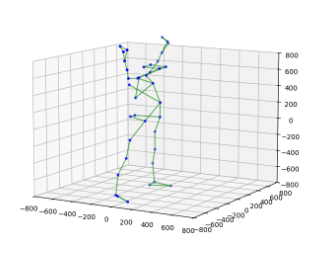
\includegraphics[width=\linewidth]{figures/VICON-39-joints-exercise0-frame-3d-plot.png}
        \vspace{0.2cm}
        \small (a) Full 39-joint Vicon capture
    \end{minipage}
    \hfill
    \begin{minipage}[t]{0.48\textwidth}
        \centering
        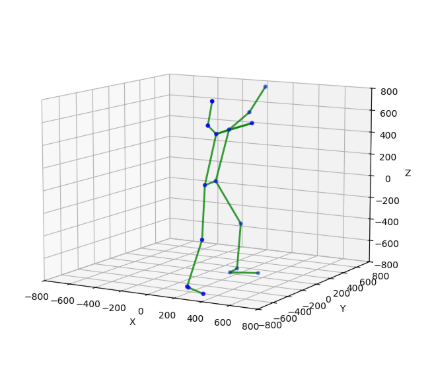
\includegraphics[width=\linewidth]{figures/VICON-17-COCO-joints-exercise0-frame-3d-plot.png}
        \vspace{0.2cm}
        \small (b) Mapped 17-joint representation
    \end{minipage}
    \vspace{0.4cm}
    \caption{Example 3D Vicon captures showing the original marker-rich representation and the reduced 17-joint representation used in the thesis pipeline.}
    \label{fig:vicon-comparison}
\end{figure}

\section{Quantitative Analysis}
The quantitative analysis evaluates the framework across four distinct training configurations to isolate the impact of each architectural component. We report standard categorical metrics (accuracy, precision, recall, and F1-score) to evaluate binary correctness decisions, alongside the automatically calibrated decision threshold for each exercise. 

Because the Siamese network architecture regresses a continuous similarity score rather than predicting a discrete class label, the \textbf{threshold} serves as the explicit decision boundary. If a patient's execution score meets or exceeds this calibrated value, the movement is classified as correct. Notably, this boundary is dynamically calibrated during the validation phase to maximize the F1-score, accommodating the unique biomechanical variance and baseline difficulty inherent to each specific exercise.

To rigorously test the system's capabilities and generalization, the evaluation is broken down into the following configurations:
\begin{itemize}
    \item \textbf{Baseline Variant} (Table \ref{tab:baseline}): The standard Siamese ST-GAT architecture without auxiliary temporal alignment or spatial penalties.
    \item \textbf{Phase-Aware Variant without ROM} (Table \ref{tab:phase-aware-no-rom}): Introduces the temporal phase-alignment module to synchronize varying execution speeds.
    \item \textbf{Phase-Aware Variant with ROM} (Table \ref{tab:phase-aware-rom}): Adds Range-of-Motion regularization to explicitly penalize partial-range executions.
    \item \textbf{Leave-One-Subject-Out (LOSO)} (Table \ref{tab:loso-metrics}): Applies the most robust configuration (Phase-Aware with ROM) under strict cross-subject validation to test true generalization against entirely unseen patients.
\end{itemize}

\begin{table}[htbp]
    \centering
    \caption{Baseline variant.}
    \label{tab:baseline}
    \begin{tabularx}{0.8\textwidth}{@{} c c c c c c @{}}
        \toprule
        \textbf{Ex. ID} & \textbf{Threshold} & \textbf{Accuracy} & \textbf{Precision} & \textbf{Recall} & \textbf{F1} \\
        \midrule
        1  & -0.415 & 0.850 & 0.769 & 1.000 & 0.870 \\
        2  &  0.952 & 1.000 & 1.000 & 1.000 & 1.000 \\
        3  & -0.199 & 1.000 & 1.000 & 1.000 & 1.000 \\
        4  &  0.481 & 0.800 & 0.714 & 1.000 & 0.833 \\
        5  & -0.506 & 1.000 & 1.000 & 1.000 & 1.000 \\
        6  &  0.663 & 0.950 & 0.909 & 1.000 & 0.952 \\
        7  &  0.793 & 0.900 & 1.000 & 0.800 & 0.889 \\
        8  & -0.255 & 1.000 & 1.000 & 1.000 & 1.000 \\
        9  &  0.990 & 0.800 & 0.750 & 0.900 & 0.818 \\
        10 &  0.924 & 1.000 & 1.000 & 1.000 & 1.000 \\
        \bottomrule
    \end{tabularx}
\end{table}

\begin{table}[htbp]
    \centering
    \caption{Phase-aware variant without ROM regularization.}
    \label{tab:phase-aware-no-rom}
    \begin{tabularx}{0.8\textwidth}{@{} c c c c c c @{}}
        \toprule
        \textbf{Ex. ID} & \textbf{Threshold} & \textbf{Accuracy} & \textbf{Precision} & \textbf{Recall} & \textbf{F1} \\
        \midrule
        1  &  0.758 & 1.000 & 1.000 & 1.000 & 1.000 \\
        2  &  0.822 & 1.000 & 1.000 & 1.000 & 1.000 \\
        3  & -0.151 & 0.900 & 0.900 & 0.900 & 0.900 \\
        4  &  0.864 & 0.900 & 0.833 & 1.000 & 0.909 \\
        5  & -0.539 & 0.900 & 0.833 & 1.000 & 0.909 \\
        6  &  0.697 & 0.950 & 0.909 & 1.000 & 0.952 \\
        7  &  0.956 & 1.000 & 1.000 & 1.000 & 1.000 \\
        8  &  0.601 & 1.000 & 1.000 & 1.000 & 1.000 \\
        9  &  0.754 & 0.500 & 0.500 & 1.000 & 0.667 \\
        10 &  0.880 & 1.000 & 1.000 & 1.000 & 1.000 \\
        \bottomrule
    \end{tabularx}
\end{table}

\begin{table}[htbp]
    \centering
    \caption{Phase-aware variant with ROM (Range-of-Motion) regularization.}
    \label{tab:phase-aware-rom}
    \begin{tabularx}{0.8\textwidth}{@{} c c c c c c @{}}
        \toprule
        \textbf{Ex. ID} & \textbf{Threshold} & \textbf{Accuracy} & \textbf{Precision} & \textbf{Recall} & \textbf{F1} \\
        \midrule
        1  &  0.886 & 0.900 & 0.833 & 1.000 & 0.909 \\
        2  &  0.060 & 1.000 & 1.000 & 1.000 & 1.000 \\
        3  &  0.233 & 0.850 & 1.000 & 0.700 & 0.824 \\
        4  &  0.801 & 0.900 & 0.833 & 1.000 & 0.909 \\
        5  & -0.663 & 0.950 & 0.909 & 1.000 & 0.952 \\
        6  &  0.027 & 0.850 & 0.818 & 0.900 & 0.857 \\
        7  & -0.387 & 1.000 & 1.000 & 1.000 & 1.000 \\
        8  & -0.552 & 0.600 & 0.556 & 1.000 & 0.714 \\
        9  &  0.445 & 0.800 & 0.714 & 1.000 & 0.833 \\
        10 &  0.990 & 1.000 & 1.000 & 1.000 & 1.000 \\
        \bottomrule
    \end{tabularx}
\end{table}

\begin{table}[htbp]
    \centering
    \caption{Leave-One-Subject-Out (LOSO) Aggregated Metrics per Exercise. Evaluated utilizing the Phase-Aware variant with ROM regularization.}
    \label{tab:loso-metrics}
    \begin{tabularx}{0.8\textwidth}{@{} c c c c c c @{}}
        \toprule
        \textbf{Ex. ID} & \textbf{Threshold} & \textbf{Accuracy} & \textbf{Precision} & \textbf{Recall} & \textbf{F1} \\
        \midrule
        1  &  0.532 & 0.865 & 0.816 & 1.000 & 0.891 \\
        2  &  0.506 & 0.945 & 0.914 & 1.000 & 0.951 \\
        3  &  0.645 & 0.755 & 0.724 & 0.988 & 0.821 \\
        4  &  0.602 & 0.760 & 0.705 & 0.990 & 0.814 \\
        5  &  0.365 & 0.910 & 0.881 & 0.960 & 0.916 \\
        6  &  0.499 & 0.965 & 0.949 & 0.990 & 0.968 \\
        7  &  0.423 & 0.920 & 0.890 & 1.000 & 0.935 \\
        8  &  0.819 & 0.800 & 0.772 & 1.000 & 0.856 \\
        9  &  0.505 & 0.830 & 0.803 & 0.990 & 0.872 \\
        10 &  0.596 & 0.795 & 0.750 & 0.990 & 0.844 \\
        \bottomrule
    \end{tabularx}
\end{table}

While the aggregated metrics across the subject-wise splits (Tables \ref{tab:baseline} -- \ref{tab:phase-aware-rom}) show high initial performance, a granular analysis reveals the critical importance of the architectural enhancements. Specifically, the baseline model frequently struggles to accurately assess videos containing partial-range executions, where a patient maintains correct anatomical posture but prematurely terminates the repetition. 

The introduction of the phase-aware variant, specifically coupled with ROM regularization, explicitly addresses this clinical nuance. By actively penalizing incomplete spatial trajectories, the ROM-regularized model significantly reduces false positives. In a real-world rehabilitation context, this behavior is paramount to ensure patients are not incorrectly rewarded for incomplete routines.

Furthermore, Table \ref{tab:loso-metrics} validates the true generalizability of the framework. Evaluated under strict Leave-One-Subject-Out (LOSO) conditions—which prevents the network from memorizing patient-specific physical traits—the metrics naturally exhibit a slight, expected decrease compared to standard splits. However, maintaining high average F1-scores across entirely unseen subjects confirms that the network has successfully learned to generalize underlying biomechanical movement patterns, effectively solving the identity leakage problem.\section{Quantitative Analysis}
The quantitative analysis evaluates the framework across four distinct training configurations to isolate the impact of each architectural component. We report standard categorical metrics (accuracy, precision, recall, and F1-score) to evaluate binary correctness decisions, alongside the automatically calibrated decision threshold for each exercise. 

Because the Siamese network architecture regresses a continuous similarity score rather than predicting a discrete class label, the \textbf{threshold} serves as the explicit decision boundary. If a patient's execution score meets or exceeds this calibrated value, the movement is classified as correct. Notably, this boundary is dynamically calibrated during the validation phase to maximize the F1-score, accommodating the unique biomechanical variance and baseline difficulty inherent to each specific exercise.

To rigorously test the system's capabilities and generalization, the evaluation is broken down into the following configurations:
\begin{itemize}
    \item \textbf{Baseline Variant} (Table \ref{tab:baseline}): The standard Siamese ST-GAT architecture without auxiliary temporal alignment or spatial penalties.
    \item \textbf{Phase-Aware Variant without ROM} (Table \ref{tab:phase-aware-no-rom}): Introduces the temporal phase-alignment module to synchronize varying execution speeds.
    \item \textbf{Phase-Aware Variant with ROM} (Table \ref{tab:phase-aware-rom}): Adds Range-of-Motion regularization to explicitly penalize partial-range executions.
    \item \textbf{Leave-One-Subject-Out (LOSO)} (Table \ref{tab:loso-metrics}): Applies the most robust configuration (Phase-Aware with ROM) under strict cross-subject validation to test true generalization against entirely unseen patients.
\end{itemize}

\begin{table}[htbp]
    \centering
    \caption{Baseline variant.}
    \label{tab:baseline}
    \begin{tabularx}{0.8\textwidth}{@{} c c c c c c @{}}
        \toprule
        \textbf{Ex. ID} & \textbf{Threshold} & \textbf{Accuracy} & \textbf{Precision} & \textbf{Recall} & \textbf{F1} \\
        \midrule
        1  & -0.415 & 0.850 & 0.769 & 1.000 & 0.870 \\
        2  &  0.952 & 1.000 & 1.000 & 1.000 & 1.000 \\
        3  & -0.199 & 1.000 & 1.000 & 1.000 & 1.000 \\
        4  &  0.481 & 0.800 & 0.714 & 1.000 & 0.833 \\
        5  & -0.506 & 1.000 & 1.000 & 1.000 & 1.000 \\
        6  &  0.663 & 0.950 & 0.909 & 1.000 & 0.952 \\
        7  &  0.793 & 0.900 & 1.000 & 0.800 & 0.889 \\
        8  & -0.255 & 1.000 & 1.000 & 1.000 & 1.000 \\
        9  &  0.990 & 0.800 & 0.750 & 0.900 & 0.818 \\
        10 &  0.924 & 1.000 & 1.000 & 1.000 & 1.000 \\
        \bottomrule
    \end{tabularx}
\end{table}

\begin{table}[htbp]
    \centering
    \caption{Phase-aware variant without ROM regularization.}
    \label{tab:phase-aware-no-rom}
    \begin{tabularx}{0.8\textwidth}{@{} c c c c c c @{}}
        \toprule
        \textbf{Ex. ID} & \textbf{Threshold} & \textbf{Accuracy} & \textbf{Precision} & \textbf{Recall} & \textbf{F1} \\
        \midrule
        1  &  0.758 & 1.000 & 1.000 & 1.000 & 1.000 \\
        2  &  0.822 & 1.000 & 1.000 & 1.000 & 1.000 \\
        3  & -0.151 & 0.900 & 0.900 & 0.900 & 0.900 \\
        4  &  0.864 & 0.900 & 0.833 & 1.000 & 0.909 \\
        5  & -0.539 & 0.900 & 0.833 & 1.000 & 0.909 \\
        6  &  0.697 & 0.950 & 0.909 & 1.000 & 0.952 \\
        7  &  0.956 & 1.000 & 1.000 & 1.000 & 1.000 \\
        8  &  0.601 & 1.000 & 1.000 & 1.000 & 1.000 \\
        9  &  0.754 & 0.500 & 0.500 & 1.000 & 0.667 \\
        10 &  0.880 & 1.000 & 1.000 & 1.000 & 1.000 \\
        \bottomrule
    \end{tabularx}
\end{table}

\begin{table}[htbp]
    \centering
    \caption{Phase-aware variant with ROM (Range-of-Motion) regularization.}
    \label{tab:phase-aware-rom}
    \begin{tabularx}{0.8\textwidth}{@{} c c c c c c @{}}
        \toprule
        \textbf{Ex. ID} & \textbf{Threshold} & \textbf{Accuracy} & \textbf{Precision} & \textbf{Recall} & \textbf{F1} \\
        \midrule
        1  &  0.886 & 0.900 & 0.833 & 1.000 & 0.909 \\
        2  &  0.060 & 1.000 & 1.000 & 1.000 & 1.000 \\
        3  &  0.233 & 0.850 & 1.000 & 0.700 & 0.824 \\
        4  &  0.801 & 0.900 & 0.833 & 1.000 & 0.909 \\
        5  & -0.663 & 0.950 & 0.909 & 1.000 & 0.952 \\
        6  &  0.027 & 0.850 & 0.818 & 0.900 & 0.857 \\
        7  & -0.387 & 1.000 & 1.000 & 1.000 & 1.000 \\
        8  & -0.552 & 0.600 & 0.556 & 1.000 & 0.714 \\
        9  &  0.445 & 0.800 & 0.714 & 1.000 & 0.833 \\
        10 &  0.990 & 1.000 & 1.000 & 1.000 & 1.000 \\
        \bottomrule
    \end{tabularx}
\end{table}

\begin{table}[htbp]
    \centering
    \caption{Leave-One-Subject-Out (LOSO) Aggregated Metrics per Exercise. Evaluated utilizing the Phase-Aware variant with ROM regularization.}
    \label{tab:loso-metrics}
    \begin{tabularx}{0.8\textwidth}{@{} c c c c c c @{}}
        \toprule
        \textbf{Ex. ID} & \textbf{Threshold} & \textbf{Accuracy} & \textbf{Precision} & \textbf{Recall} & \textbf{F1} \\
        \midrule
        1  &  0.532 & 0.865 & 0.816 & 1.000 & 0.891 \\
        2  &  0.506 & 0.945 & 0.914 & 1.000 & 0.951 \\
        3  &  0.645 & 0.755 & 0.724 & 0.988 & 0.821 \\
        4  &  0.602 & 0.760 & 0.705 & 0.990 & 0.814 \\
        5  &  0.365 & 0.910 & 0.881 & 0.960 & 0.916 \\
        6  &  0.499 & 0.965 & 0.949 & 0.990 & 0.968 \\
        7  &  0.423 & 0.920 & 0.890 & 1.000 & 0.935 \\
        8  &  0.819 & 0.800 & 0.772 & 1.000 & 0.856 \\
        9  &  0.505 & 0.830 & 0.803 & 0.990 & 0.872 \\
        10 &  0.596 & 0.795 & 0.750 & 0.990 & 0.844 \\
        \bottomrule
    \end{tabularx}
\end{table}

While the aggregated metrics across the subject-wise splits (Tables \ref{tab:baseline} -- \ref{tab:phase-aware-rom}) show high initial performance, a granular analysis reveals the critical importance of the architectural enhancements. Specifically, the baseline model frequently struggles to accurately assess videos containing partial-range executions, where a patient maintains correct anatomical posture but prematurely terminates the repetition. 

The introduction of the phase-aware variant, specifically coupled with ROM regularization, explicitly addresses this clinical nuance. By actively penalizing incomplete spatial trajectories, the ROM-regularized model significantly reduces false positives. In a real-world rehabilitation context, this behavior is paramount to ensure patients are not incorrectly rewarded for incomplete routines.

Furthermore, Table \ref{tab:loso-metrics} validates the true generalizability of the framework. Evaluated under strict Leave-One-Subject-Out (LOSO) conditions—which prevents the network from memorizing patient-specific physical traits—the metrics naturally exhibit a slight, expected decrease compared to standard splits. However, maintaining high average F1-scores across entirely unseen subjects confirms that the network has successfully learned to generalize underlying biomechanical movement patterns, effectively solving the identity leakage problem.


\subsection{Stream Importance and Ablation Studies}
To rigorously isolate the contribution of each architectural component and validate the complexity of the final KinetoCheck pipeline, we conducted a systematic ablation study. By incrementally enabling specific modules and feature strategies, we measured their direct impact on the model's classification metrics and real-world clinical robustness. 

The ablation experiments were structured around three primary architectural axes:

\begin{itemize}
    \item \textbf{Ablation 1: Kinematic Feature Representation (Baseline XYZ vs. 12-Channel Augmented):} 
    The network was initially evaluated using only raw 3D spatial coordinates (the Baseline variant). We compared this against the augmented 12-channel feature representation, which incorporates velocity, acceleration, joint angles, and normalized bone ratios. Results indicate that the angle-based feature strategy provides consistent performance gains. By explicitly feeding the network temporal derivatives (velocity and acceleration), the model becomes significantly more adept at identifying unstable trajectories, jitters, and compensatory movements that static XYZ coordinates alone fail to capture.
    
    \item \textbf{Ablation 2: Temporal Phase-Alignment (Baseline vs. Phase-Aware):} 
    We evaluated the network with and without the multi-task Frame Decoder and temporal interpolation modules. In the strict baseline configuration, the Siamese network rigidly compares spatial frames, inadvertently penalizing patients simply for executing a therapeutic movement slower than the healthy expert template. Introducing the phase-aware variant resolves this temporal misalignment, drastically improving precision and recall metrics while ensuring the generated ``Ghost Skeleton'' remains perfectly synchronized with the user's continuous progression.
    
    \item \textbf{Ablation 3: Range-of-Motion (ROM) Regularization:} 
    Finally, we isolated the impact of the ROM penalty by comparing the phase-aware model with and without this auxiliary loss function (comparing Table \ref{tab:phase-aware-no-rom} against Table \ref{tab:phase-aware-rom}). The ablation reveals that ROM regularization is crucial for reducing false positives on partial-range executions. Without this penalty, the network occasionally classifies shallow, incomplete movements as ``correct'' simply because the user maintained proper anatomical posture. The ROM penalty explicitly forces the spatial attention layers to verify the full amplitude of the repetition, preventing the system from rewarding truncated exercises.
\end{itemize}

Ultimately, these ablations demonstrate that while a standard Siamese ST-GAT can achieve adequate baseline classification, the synergistic combination of 12-channel kinematics, phase-awareness, and ROM regularization is strictly necessary to produce a robust, clinically viable rehabilitation assessment tool.

\section{Qualitative Analysis}
Visual inspection of the feedback overlays provides qualitative evidence that the model highlights clinically meaningful error locations. Figure~\ref{fig:annotated-video} shows example visualizations for an execution, showcasing the visual feedback at two different time steps. 

\begin{figure}[H]
    \centering
    % First sub-figure
    \begin{minipage}[t]{0.48\textwidth}
        \centering
        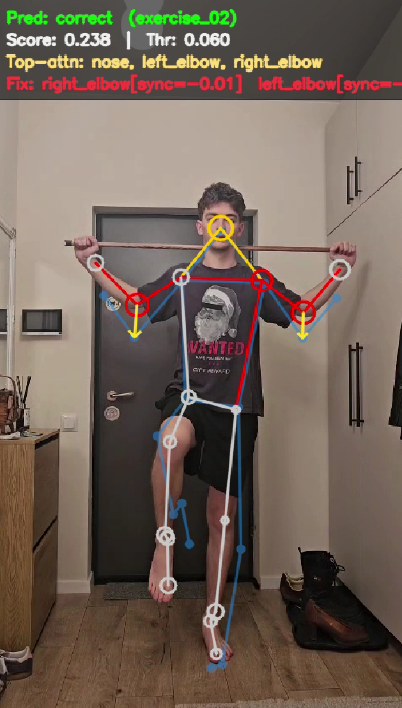
\includegraphics[width=\linewidth]{figures/ex02_start.png}
        \vspace{0.2cm} % Adds a tiny bit of space between image and text
        
        \small (a) Starting point of the movement
    \end{minipage}
    \hfill
    % Second sub-figure
    \begin{minipage}[t]{0.48\textwidth}
        \centering
        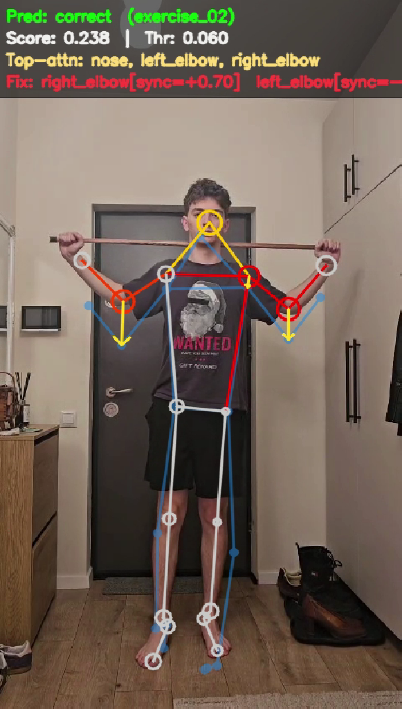
\includegraphics[width=\linewidth]{figures/ex02_halfway.png}
        \vspace{0.2cm}
        
        \small (b) Halfway through the movement
    \end{minipage}
    
    % Main figure caption
    \vspace{0.4cm} % Adds space before the main caption
    \caption{Example Annotated Video with 2 skeleton overlays: blue for the template skeleton and white/yellow/red for the MediaPipe skeleton, with corresponding colors for the worst joints.}
    \label{fig:annotated-video}
\end{figure}

\subsection{End-to-End Clinical Feedback Walkthrough}
To demonstrate the practical utility of the KinetoCheck pipeline, it is useful to examine the exact system behavior and data artifacts generated during a single rehabilitation session. Consider a scenario where a user uploads a video using the "System auto detect" feature. In this specific case, the user attempts Exercise 01 but executes it incorrectly.
\begin{figure}[H]
\centering
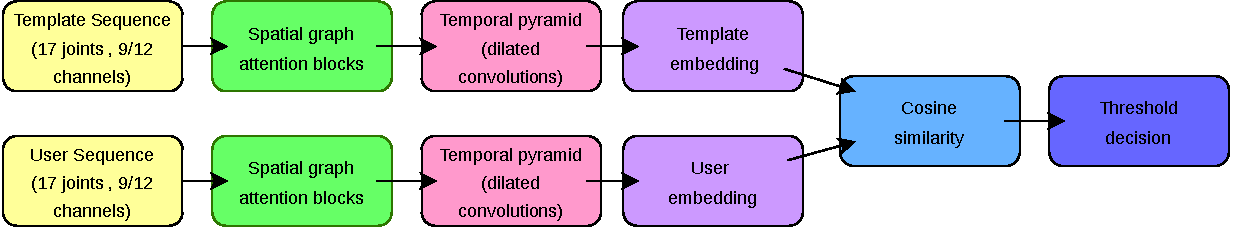
\includegraphics[width=1\textwidth]{figures/Siamese_ST-GAT.pdf}
\caption{Siamese ST-GAT with temporal pyramid architecture used in the thesis.}
\label{fig:siamese-stgat-architecture}
\end{figure}

The baseline model doesn't expose the correct skeleton execution, while the phase-aware variant provides additional metadata that improves the interpretability of the feedback.

\begin{figure}[H]
    \centering
    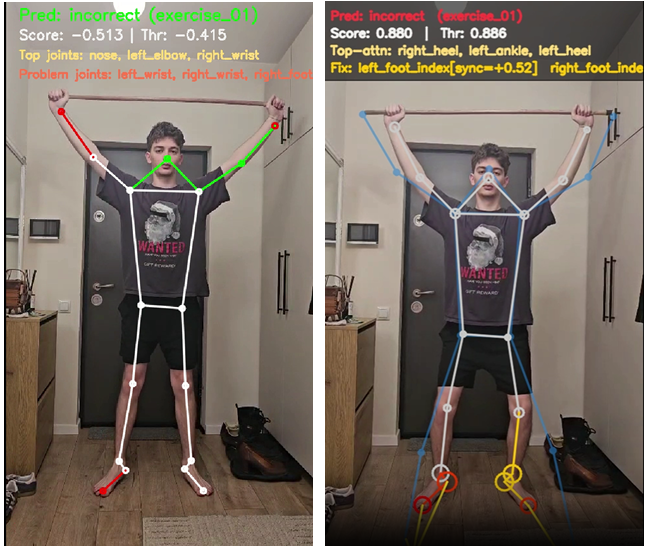
\includegraphics[width=1\textwidth]{figures/feedback_comparison.png}
    \caption{Example feedback visualizations: baseline (left) vs phase-aware (right).}
    \label{fig:feedback-comparison}
\end{figure}
Upon processing the video, the inference engine evaluates the 12-channel kinematic sequence against all ten exercise-specific ST-GAT models concurrently. Each model computes its own similarity score and compares it against its calibrated decision threshold. The system then ranks the outputs based on the classification margin (the distance between the score and the threshold). The engine packages these insights—along with localized joint error metrics—into a structured, machine-readable JSON report. A representation of this output payload is provided in Listing~\ref{lst:json-output}.

\begin{lstlisting}[language=java, caption=Generated JSON report showcasing multi-model auto-detection and joint-level insights., label=lst:json-output, frame=single, numbers=left]
{
  "video": ".../ex1-2-rep-inc.mp4",
  "annotated_video": ".../ex1-2-rep-inc_annotated.mp4",
  "num_frames": 236,
  "worst_joints": [
    {
      "joint": "right_elbow",
      "joint_index": 4,
      "deviation": 0.003,
      "importance": 0.457,
      "problem_score": 0.966
    },
    {
      "joint": "left_elbow",
      "joint_index": 3,
      "deviation": 0.003,
      "importance": 0.476,
      "problem_score": 0.981
    },
    { "..." : "..." }
  ],
  "best": {
    "exercise_id": 1,
    "exercise_name": "exercise_02",
    "score": 0.980,
    "threshold": 0.060,
    "margin": 0.920,
    "predicted_label": "correct"
  },
  "all": [
    {
      "exercise_name": "exercise_02",
      "score": 0.980,
      "threshold": 0.060,
      "margin": 0.920,
      "predicted_label": "correct"
    },
    {
      "exercise_name": "exercise_01",
      "score": 0.880,
      "threshold": 0.886,
      "margin": -0.006,
      "predicted_label": "incorrect"
    },
    { "..." : "..." }
  ]
}
\end{lstlisting}

As illustrated in Listing~\ref{lst:json-output}, the model does not merely return a binary pass/fail state. The \texttt{all} array reveals the multi-task evaluation: while the system identified the movement as a passing execution of Exercise 02 (yielding the highest positive margin of 0.920), it correctly flagged the execution as incorrect when evaluated strictly against the Exercise 01 template (failing the threshold by a margin of $-0.006$).

Furthermore, the payload isolates the anatomical source of the error within the \texttt{worst\_joints} array. In this execution, the left and right elbows are explicitly flagged as the primary components degrading the similarity score. The \texttt{importance} metric is derived directly from the Spatial Graph Attention (ST-GAT) weights, while the \texttt{deviation} magnitude is provided by the auxiliary Frame Decoder.

The ASP.NET web interface parses this payload, mapping the data to the \texttt{UploadStatistics} and \texttt{JointInsight} database entities. It then renders the user dashboard, overlaying the ghost skeleton on the video and drawing explicit visual attention to the failing joints. This pipeline successfully transforms complex, multi-model neural network outputs into a localized, interpretable, and highly actionable corrective cue for the patient.

\subsection{Longitudinal Patient Tracking and Analytics}
While isolated frame-by-frame feedback is critical for immediate postural correction, the ultimate goal of a physical rehabilitation platform is to quantify recovery over time. To serve both the patient and the overseeing physical therapist, KinetoCheck aggregates the \texttt{AnalysisHistoryEntry} database records into a comprehensive clinical statistics dashboard.

As shown in Figure~\ref{fig:app-statistics}, the system processes historical uploads to visualize the patient’s recovery trajectory. By aggregating metrics such as the total volume of exercises performed, the overall success rate, and a time-series plot of recent similarity scores, the platform provides objective proof of motor function improvement. Furthermore, by isolating the most frequently failing anatomical joints across all sessions, the system allows therapists to identify chronic biomechanical weaknesses and adjust the patient’s training regimen accordingly.

\begin{figure}[H]
    \centering
    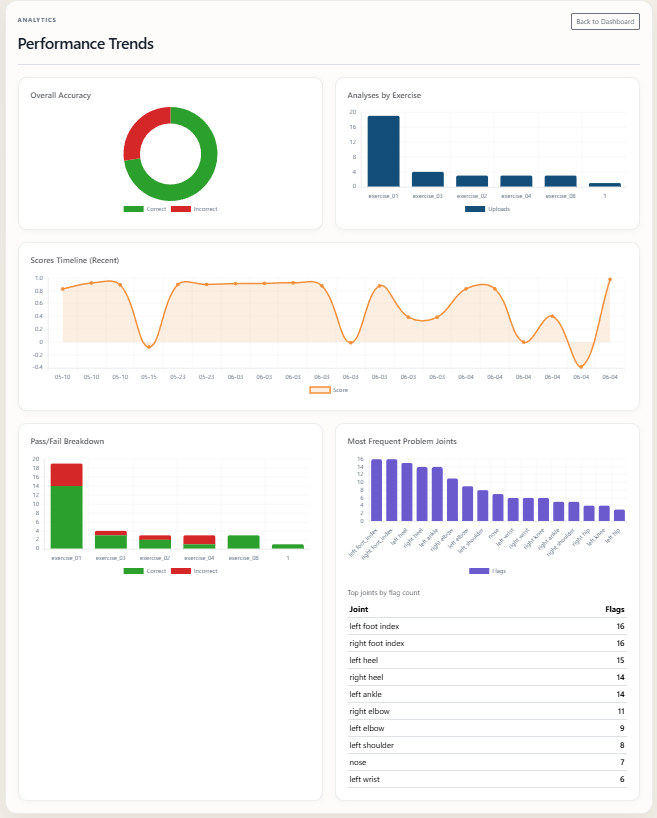
\includegraphics[width=0.85\textwidth]{figures/app_statistics.png}
    \caption{The KinetoCheck statistics dashboard, providing longitudinal analytics, success rates, and chronic joint error aggregations for long-term rehabilitation tracking.}
    \label{fig:app-statistics}
\end{figure}

\section{Generalization Challenges and Limitations}
Although results are promising, several limitations remain important to acknowledge. The primary limitation is dataset size. UI-PRMD contains 1,980 sequences across 10 subjects and 10 exercises, which is modest compared to large-scale action recognition benchmarks.

As discussed in Chapter 2, attention-based explanations should be interpreted cautiously. High attention does not automatically imply causal biomechanical error. The feedback overlays provide a useful heuristic but are not a substitute for expert clinical judgment.

\subsection{Error Analysis and Known Failure Modes}
While quantitative metrics show high performance, error analysis reveals specific edge cases where the pipeline struggles. Understanding these is critical for safe clinical deployment. The primary failure modes include:

\begin{itemize}
    \item \textbf{Severe Self-Occlusion:} During deep rotation or limb crossing, MediaPipe may lose track of distal joints. While short dropouts ($< 2$ frames) are forward-filled, extended occlusions freeze joint coordinates. The ST-GAT model interprets this rigidity as a biomechanical error, triggering false positives.
    \item \textbf{Depth Ambiguity in 2D Projections:} Extracting 3D coordinates from 2D RGB causes depth compression for movements parallel to the camera axis. The resulting drop in Z-coordinate variance can cause the model to underestimate Range of Motion (ROM) and penalize correct executions.
    \item \textbf{Clothing-Induced Landmark Jitter:} Loose clothing can confuse pose extraction, causing rapid landmark jitter. Despite Gaussian temporal smoothing, extreme high-frequency jitter is sometimes encoded by short-term convolutional kernels (\texttt{kernel size=3}) as instability, negatively skewing the similarity score.
\end{itemize}

These failure modes underscore the necessity of "Joints of Attention" overlays. Visualizing the ghost skeleton and highlighting problematic joints allows users to immediately recognize if a low score stems from genuine form error or a temporary pose-extraction failure.

% ==========================================
% CHAPTER 6: CONCLUSIONS
% ==========================================
\chapter{Conclusions and Future Directions}
\label{chap:conclusions}

This chapter summarizes the contributions of the thesis and reflects on their significance within the broader context of rehabilitation technology and machine learning. It recapitulates how the work addresses the research gaps identified in Chapter 2, consolidates the key findings from the experimental validation in Chapter 5, and outlines promising directions for future research and practical deployment.

\section{Thesis Contributions Summary}
This thesis has developed KinetoCheck, a comprehensive framework for interpretable, subject-invariant rehabilitation exercise quality assessment. The key contributions span four complementary areas:

\begin{itemize}
    \item \textbf{Representation and Model Design:} Proposed and implemented systematic geometric normalization and preprocessing strategies that enable reliable transfer from laboratory motion-capture training (UI-PRMD) to real-world RGB-based deployment via MediaPipe. Organized the implementation around feature strategies, allowing the training pipeline to switch between baseline XYZ features and angle-augmented features.
    
    \item \textbf{Subject-Invariant Training and Evaluation:} Applied rigorous subject-level split protocols (subject-wise and Leave-One-Subject-Out) to ensure that models generalize to unseen subjects rather than overfitting to subject-specific body characteristics. Centralized the training loop in a reusable trainer so that baseline, factory-based, and phase-aware runs share the same evaluation and checkpointing logic.
    
    \item \textbf{Interpretability and Clinical Actionability:} Extracted and operationalized attention-based explanations as joint-level feedback overlays (Joints of Attention), providing localized corrective hints that guide users and therapists toward movement improvements. Designed a standalone analytics service that aggregates individual inference results into user-level progress metrics, enabling longitudinal tracking.
    
    \item \textbf{End-to-End System Integration:} Implemented a modular, maintainable system that separates training, inference, and reporting components. Engineered checkpoint management and factory-pattern loading that gracefully switches between baseline, phase-aware, and ROM-regularized model variants. Implemented comprehensive error detection and user-transparent fallback behaviors for common failure modes.
\end{itemize}

\section{Key Empirical Findings}
The experimental validation in Chapter 5 yields several important findings across three dimensions:

\begin{itemize}
    \item \textbf{Performance Improvements:} The comparison in Chapter 5 shows distinct performance differences between the baseline and phase-aware variants. LOSO evaluation, when used, produces more conservative estimates than subject-wise splits, confirming the necessity of rigorous split protocols.
    
    \item \textbf{Interpretability Validation:} Qualitative analysis of feedback overlays demonstrates that the model highlights clinically meaningful error locations, lending credibility to the interpretability claims. The phase-aware variant exposes additional correction metadata, which improves the readability of the feedback presented to the user.
    
    \item \textbf{Generalization and Robustness:} Subject-invariant training via geometric normalization and augmentation effectively mitigates identity leakage. ROM regularization provides robustness against partial-range executions, reducing false positives in clinical scenarios where full range-of-motion is medically necessary.
\end{itemize}

\section{Limitations and Honest Assessment}
While the contributions are substantial, several limitations warrant explicit discussion. The UI-PRMD dataset is modest in scale; future work should validate generalization across broader demographic ranges and exercise repertoires. Furthermore, the thesis has focused primarily on offline evaluation from pre-recorded videos. Real-time performance, user interface design, and clinician feedback integration remain important practical considerations.

Finally, as discussed in Chapter 2, attention mechanisms are heuristics, not causal explanations. The feedback overlays provide useful decision support but should not be interpreted as definitive biomechanical diagnoses.

\section{Future Research Directions}
Several promising directions emerge from this work:

\begin{itemize}
    \item \textbf{Dataset Expansion and Clinical Diversity:} While the UI-PRMD dataset provided a strong foundational benchmark, gathering a larger, more diverse dataset—particularly one including patients with documented musculoskeletal pathologies—would further enhance the model's generalization capabilities and clinical reliability.
    
    \item \textbf{Real-Time Inference and Live Feedback:} Transitioning the current offline, video-based pipeline into a real-time streaming architecture. By utilizing a sliding temporal window over live camera feeds, the system could provide immediate, intra-repetition postural corrections, significantly enhancing the interactive telerehabilitation experience.
    
    \item \textbf{Automated Repetition Segmentation and Counting:} Extending the temporal alignment and phase-aware modules to process continuous, unsegmented video streams. This would allow the system to automatically count repetitions and evaluate kinematic fatigue over the course of a full rehabilitation set, rather than evaluating isolated, single repetitions.
    \item \textbf{Multi-Modal Integration:} Extending the framework to fuse RGB and depth data to improve robustness in challenging lighting or occlusion scenarios.
\end{itemize}

\section{Concluding Remarks}
This thesis has presented a comprehensive framework for interpretable, subject-invariant rehabilitation exercise assessment. By combining rigorous machine learning practices with practical system engineering, KinetoCheck demonstrates that high-performance rehabilitation AI is achievable without sacrificing clinical transparency.

As rehabilitation technology continues to evolve, this thesis contributes both concrete tools and methodological insights that will hopefully inform future work in clinical AI. The code, data, and detailed documentation provided are offered in the spirit of open science, with the hope that they accelerate progress in rehabilitation technology.
%\addcontentsline{toc}{chapter}{Concluzii}
%\addcontentsline{toc}{chapter}{Conclusions}


\bibliography{references}

\end{document}